%---------------
%╔═╗╔═╗╔╦╗╦ ╦╔═╗
%╚═╗║╣  ║ ║ ║╠═╝
%╚═╝╚═╝ ╩ ╚═╝╩  
%---------------

% language setup
\newcommand{\docLanguage}{ngerman}
\RequirePackage{mmap}%
% DOCUMENT SETUP
\documentclass[oneside]{htwg-report} % remove oneside for printing version

% encoding setup
% T1 font encoding for languages that use a latin alphabet
\usepackage[T1]{fontenc} 

% enhanced input encoding handling - utf8 for äÄüÜöÖß...
\usepackage[utf8]{inputenc}

% glossary
\usepackage[style=long,nonumberlist,toc]{glossaries}
\loadglsentries{vorwort/glossentries}

% floating prevention packages
\usepackage{float}    % used with [H] positioning parameter

\usepackage{filecontents}
\usepackage{graphicx}

\addbibresource{./bib/report.bib}

% Caption
\usepackage{caption}
\DeclareCaptionFont{white}{\color{white}}
\DeclareCaptionFormat{listing}{\colorbox{htwg-teal}{\parbox{\textwidth}{#1#2#3}}}
\DeclareCaptionFormat{figure}{\colorbox{htwg-teal}{\parbox{\textwidth}{#1#2#3}}}
\DeclareCaptionFormat{table}{\colorbox{htwg-teal}{\parbox{\textwidth}{#1#2#3}}}
\captionsetup[lstlisting]{format=listing,labelfont=white,textfont=white}
\captionsetup[figure]{format=listing,labelfont=white,textfont=white}
\captionsetup[table]{format=listing,labelfont=white,textfont=white}

\newcommand{\repeatcaption}[2]{%
  \renewcommand{\thefigure}{\ref{#1}}%
  \captionsetup{list=no}%
  \caption{#2 (Wiederholung von Seite \pageref{#1})}%
}

% to large table
\usepackage{booktabs}

% enumeration
\usepackage{enumitem}
% tabular extension tabularx
\usepackage{tabularx}

% Listing configs
\usepackage{listings}
% Matlab Syntax Highlighting
\colorlet{keyword}{blue!100!black!80}
\colorlet{STD}{red}
\colorlet{comment}{green!90!black!90}
\definecolor{mygreen}{rgb}{0,0.6,0}
\definecolor{mygray}{rgb}{0.5,0.5,0.5}
\definecolor{mymauve}{rgb}{0.58,0,0.82}


\lstdefinestyle{LATEX}{ 
  language     = [LaTeX]{TeX},
  basicstyle   = \footnotesize \ttfamily,
  keywordstyle = [1]\color{keyword}\bfseries,
  keywordstyle = [2]\color{comment}\bfseries,
  commentstyle = \color{mygray}\itshape,
  %backgroundcolor=\color{white},   % choose the background color; you must add \usepackage{color} 
                                   % or \usepackage{xcolor}
  basicstyle=\footnotesize,        		   % the size of the fonts that are used for the code
  breakatwhitespace=false,         % sets if automatic breaks should only happen at whitespace
  columns=fullflexible,            % copy pasteable listings
  breaklines=true,                 % sets automatic line breaking
  captionpos=c,                    % sets the caption-position to bottom
  extendedchars=true,              % lets you use non-ASCII characters; for 8-bits encodings only,
                                   % does not work with UTF-8
  frame=single,                    % adds a frame around the code
  keepspaces=true,                 % keeps spaces in text, useful for keeping indentation of code
                                   % (possibly needs columns=flexible)
  numbers=left,                    % where to put the line-numbers; possible values are 
                                   % (none, left, right)
  numbersep=4pt,                   % how far the line-numbers are from the code
  numberstyle=\tiny\color{mygray}, % the style that is used for the line-numbers
  rulecolor=\color{black},         % if not set, the frame-color may be changed on line-breaks
                                   % within not-black text (e.g. comments (green here))
  showspaces=false,                % show spaces everywhere adding particular underscores; it
  	                               % overrides 'showstringspaces'
  showstringspaces=false,          % underline spaces within strings only
  showtabs=false,                  % show tabs within strings adding particular underscores
  stepnumber=1,                    % the step between two line-numbers. If it's 1, each line 
                                   % will be numbered
  stringstyle=\color{mymauve},     % string literal style
  tabsize=2,                       % sets default tabsize to 2 spaces
  title=\lstname,                  % set title name
  literate=                        % replace in code
     {Ö}{{\"O}}1 
     {Ä}{{\"A}}1 
     {Ü}{{\"U}}1 
     {ß}{{\ss}}2 
     {ü}{{\"u}}1 
     {ä}{{\"a}}1 
     {ö}{{\"o}}1 
     {â}{{\^{a}}}1 
     {Â}{{\^{A}}}1 
     {ç}{{\c{c}}}1 
     {Ç}{{\c{C}}}1 
     {ğ}{{\u{g}}}1 
     {Ğ}{{\u{G}}}1 
     {ı}{{\i}}1 
     {İ}{{\.{I}}}1 
     {ş}{{\c{s}}}1 
     {Ş}{{\c{S}}}1 
}
\definecolor{javared}{rgb}{0.6,0,0} % for strings
\definecolor{javagreen}{rgb}{0.25,0.5,0.35} % comments
\definecolor{javapurple}{rgb}{0.5,0,0.35} % keywords
\definecolor{javadocblue}{rgb}{0.25,0.35,0.75} % javadoc
 
\lstset{language=Java,
basicstyle=\footnotesize,
keywordstyle=\color{javapurple}\bfseries,
stringstyle=\color{javared},
commentstyle=\color{javagreen},
morecomment=[s][\color{javadocblue}]{/**}{*/},
numbers=left,
numberstyle=\tiny\color{black},
stepnumber=1,
numbersep=10pt,
tabsize=4,
showspaces=false,
showstringspaces=false} 
% bash command line Syntax Highlighting
\lstdefinestyle{BASH_CMD}{ 
  columns=fullflexible,            % copy pasteable listings
  language=bash,
  basicstyle=\small\sffamily,
  basicstyle   = \small \ttfamily,
  keywordstyle = [1]\small \ttfamily,
  keywordstyle = [2]\small \ttfamily,
  commentstyle = \small \ttfamily,
  numbers=none,
  captionpos=b, 
  breaklines=true,
  numberstyle=\tiny,
  numbersep=3pt,
  frame=tlrb,
  columns=fullflexible,
  backgroundcolor=\color{white!20},
  linewidth=\linewidth,
  literate=                        % replace in code
     {Ö}{{\"O}}1 
     {Ä}{{\"A}}1 
     {Ü}{{\"U}}1 
     {ß}{{\ss}}2 
     {ü}{{\"u}}1 
     {ä}{{\"a}}1 
     {ö}{{\"o}}1 
     {â}{{\^{a}}}1 
     {Â}{{\^{A}}}1 
     {ç}{{\c{c}}}1 
     {Ç}{{\c{C}}}1 
     {ğ}{{\u{g}}}1 
     {Ğ}{{\u{G}}}1 
     {ı}{{\i}}1 
     {İ}{{\.{I}}}1 
     {ş}{{\c{s}}}1 
     {Ş}{{\c{S}}}1 
}
 
\lstdefinestyle{Scala}{
  frame=tb,
  language=scala,
  aboveskip=3mm,
  belowskip=3mm,
  showstringspaces=false,
  columns=flexible,
  basicstyle={\small\ttfamily},
  numbers=left,
  numberstyle=\tiny\color{gray},
  keywordstyle=\color{blue},
  commentstyle=\color{dkgreen},
  stringstyle=\color{mauve},
  frame=single,
  breaklines=true,
  breakatwhitespace=true,
  tabsize=3,
} 

%-----------------------------------------
% ╔╗ ╔═╗╔═╗╦╔╗╔  ╔╦╗╔═╗╔═╗╦ ╦╔╦╗╔═╗╔╗╔╔╦╗ 
% ╠╩╗║╣ ║ ╦║║║║   ║║║ ║║  ║ ║║║║║╣ ║║║ ║  
% ╚═╝╚═╝╚═╝╩╝╚╝  ═╩╝╚═╝╚═╝╚═╝╩ ╩╚═╝╝╚╝ ╩  
%-----------------------------------------

\begin{document}

%% 'reporttype' add background elements to the cover / front page
%% possible values are:
%% bachelor	--> B S C
%% master	--> M S C
%% other		--> none
\reporttype{bachelor}

\reporttypetext{Bachelorarbeit}

\title[Kriterien und Möglichkeiten für den Einsatz von Reaktiver Programmierung]{Kriterien und Möglichkeiten für den Einsatz von Reaktiver Programmierung}

\author{Kirill Meng}
\studentnumber{292154}
\studentemail{kimeng@htwg-konstanz.de}

\doclocation{Friedrichshafen}
\docdate{28 Februar 2019}

\makecover[]
%\setlength{\parindent}{0pt}

%% Use Roman numerals for the page numbers of the title pages and table of
%% contents.
\frontmatter
%          
%% Include an optional title page.
\begin{titlepage}
\newgeometry{hscale=0.81,vscale=0.8}

\AddToShipoutPicture*{\BackgroundImgTitelPage}

\vspace*{12\bigskipamount}


%% Print the title in htwg-teal.
{\makeatletter
\fboxsep=0pt
\colorbox{htwg-white}{\begin{minipage}[t]{145mm}
    \begin{flushleft}
        %% Print Report Type Text
        \color{htwg-teal}\Huge{\@report@typetext}
        \\
        %% Print Report Title
        \color{htwg-teal}\Huge\textbf{\@title}
    \end{flushleft}
\end{minipage}}
\makeatother}

\bigskip
\bigskip

von
%door

\bigskip
\bigskip

%% Print the name of the author.
{\makeatletter
\Large\bfseries\@author
\makeatother}

\vfill

zur Erlangung der akademischen Grades eines

\bigskip
\bigskip

{\bfseries Bachelor of Science}

in angewandter Informatik

\bigskip
\bigskip

an der Hochschule Konstanz,

\vfill

\begingroup
\renewcommand*{\arraystretch}{1}
\rowcolors{2}{white}{white}
{\makeatletter
\begin{tabular}{lll}
    Matrikelnummer: & \@student@number \\ \\
    Abgabedatum: & \@doc@date \\ \\
    1. Prüfer: & \textbf{Prof.\ Dr.\ Marko Boger} \\
    2. Prüfer: & \textbf{Dipl.-Wirt.-Inf. \ Stefan Waldmann}
\end{tabular}
\makeatother}
\endgroup

\bigskip
\bigskip
Eine elektronische Version diese Dokuments ist hier zu finden \url{https://github.com/Menkir/reactive-streams-tex/blob/master/thesis.pdf}.

%% reset page margins
\newgeometry{hscale=0.7,vscale=0.8}
\end{titlepage}


\chapter*{Ehrenwörtliche Erklärung}
\setheader{Ehrenwörtliche Erklärung}

\begingroup
{\makeatletter
Hiermit erkläre ich, \@author, geboren am 25.08.1994 in Orenburg,



\renewcommand*{\arraystretch}{1.5}
\rowcolors{2}{white}{white}
\begin{tabular}{p{50pt}p{320pt}}
         & \\
    (1) & dass ich meine Bachelorarbeit mit dem Titel: \newline \newline  
\textbf{"Kriterien und Möglichkeiten von Reaktiver Programmierung"} \newline \newline in der Fakultät Informatik unter Anleitung von Professor Dr. Marko Boger selbständig und ohne fremde Hilfe angefertigt habe und keine anderen als die angeführten Hilfen benutzt habe; \\ \\
    (2) & dass ich die Übernahme wörtlicher Zitate, von Tabellen, Zeichnungen, Bildern und Programmen aus der Literatur oder anderen Quellen (Internet) sowie die Verwendung der Gedanken anderer Autoren an den entsprechenden Stellen innerhalb der Arbeit gekennzeichnet habe. \\ \\
    (3) & dass die eingereichten Abgabe-Exemplare in Papierform und im PDF-Format vollständig übereinstimmen. \newline \newline
\end{tabular}

Ich bin mir bewusst, dass eine falsche Erklärung rechtliche Folgen haben wird.


\begin{tabular}{lp{200pt}l}
  & & \\ \\
  Konstanz, 28.02.2019 & & \@author 
\end{tabular}


\makeatother}
\endgroup



\chapter*{Abstract}
\setheader{Abstract}
In der vorliegenden Thesis soll die Frage beantwortet werden, worin Möglichkeiten und Szenarien der reaktiven Programmierung liegen. Dazu wird der Begriff zunächst differenziert und abgegrenzt. Aus der Sicht der Architektur beschreibt die reaktive Programmierung das Design eines Systems, das die vier Qualitäten des reaktiven Manifests umsetzt. Ein reaktives System muss somit widerstandsfähig, elastisch, und nachrichtenorientiert sein, damit es eine hohe Antwortbereitschaft garantieren kann. Um die Einsatzszenerien solcher Systeme aufzuzeigen, werden Erfolgsgeschichten von Unternehmen wie Netflix, PayPal und Verizon betrachtet. Der Einsatz reaktiver Systeme vereinfacht zum einen die Entwicklung der Projekte, zum anderen steigert er den Umsatz der Unternehmen.

Aus programmatischer Sicht bezeichnet die reaktive Programmierung ein Programmierparadigma. Die Technologien Reactive Streams, Futures und Spreadsheets sind mögliche Ausprägungen davon. Die Reactive Streams werden in dieser Arbeit näher untersucht und Implementierungen von verschiedenen Anbietern verglichen. Unter den Bibliotheken wie RxJava, Akka-Streams und Reactor stellt sich Letzteres als besonders einfach in der Handhabung heraus. Mithilfe dieser Bibliothek wurde anschließend eine reaktive Applikation entwickelt und hinsichtlich der Performance mit einer äquivalenten klassischen, synchronen Variante verglichen, wobei sich die reaktive Applikation als schneller erweist.  

Die reaktive Programmierung ist folglich ein Begriff, der sowohl in der Systemebene als auch in der Anwendungsebene vertreten ist. Unter den Möglichkeiten in der Anwendungsebene dominiert Reactive Streams, die in vielen Programmiersprachen und Implementierungen angeboten werden. Reactive Streams erlauben die Entwicklung von Anwendungen, die einen bedeutend höheren Durchsatz erzielen. Aus architektonischer Sicht ermöglicht die reaktive Programmierung Systeme zu entwickeln, die schnell, skalierbar und fehlertolerant sind und den Unternehmen eine Steigerung von Umsatz und Produktivität bescheren.




%
% TABLE OF CONTENTS
%
\tableofcontents
%
% Abbildungsverzeichnis
%
%
% Abbildungsverzeichnis
%
\phantomsection
\listoffigures
\addcontentsline{toc}{chapter}{Abbildungsverzeichnis}
%\thispagestyle{plain}
\newpage
%\clearpage
%
% Tabellenverzeichnis
%
%
% Tabellenverzeichnis
%
\phantomsection
\addcontentsline{toc}{chapter}{Tabellenverzeichnis}
\listoftables
%\thispagestyle{preface}
\newpage
\clearpage

%
% Listingverzeichnis
%
%
% Listingverzeichnis
%
\phantomsection
\renewcommand\lstlistingname{Listing}
\renewcommand\lstlistlistingname{Listingverzeichnis}
\lstlistoflistings
\addcontentsline{toc}{chapter}{Listingverzeichnis}
%\thispagestyle{preface}
\newpage
\clearpage

%
% Glossar
%

%
% Glossar
%
\phantomsection
\printglossary[toctitle=Glossar]
%\thispagestyle{preface}
%\newpage
%\clearpage

%% Use Arabic numerals for the page numbers of the chapters.
\mainmatter

%--------------------------
% ╔═╗╦ ╦╔═╗╔═╗╔╦╗╔═╗╦═╗╔═╗ 
% ║  ╠═╣╠═╣╠═╝ ║ ║╣ ╠╦╝╚═╗ 
% ╚═╝╩ ╩╩ ╩╩   ╩ ╚═╝╩╚═╚═╝ 
%--------------------------

\pagenumbering{arabic} 
\setcounter{page}{1} 
%
% CHAPTER Einleitung
%
\chapter{Einleitung} 
In Anwendungen ist das Paradigma der reaktiven Programmierung nicht neu, doch hält es derzeit vermehrt Einzug in das Java-Ökosystem und etabliert sich zunehmend als Standard. Die Firma doubleSlash möchte in dieser Arbeit näher untersuchen lassen wie und an welcher Stelle die reaktive Programmierung von Vorteil ist, wann sie Sinn ergibt und wann nicht.

Da reaktive Programmierung nicht nur in höheren Programmiersprachen vertreten ist, sondern auch in Systemarchitekturen, kann doubleSlash die Erkenntnisse dieser Arbeit für künftige Projekte in Zusammenarbeit mit anderen Firmen nutzen, um schnelle und skalierbare Software zu entwickeln.

Da sich die reaktive Programmierung immer größerer Beliebtheit erfreut, muss sich doubleSlash ebenfalls mit dieser Technologie beschäftigen, um auch künftig konkurrenzfähig zu bleiben. Reaktive Systeme können langfristig die klassischen Request-Response Modelle ergänzen, da die Menge der Daten im Zeitalter von Big Data immer weiter zunimmt. 

Der Begriff der reaktiven Programmierung wird in modernen Applikationen häufig genutzt. Als problematisch erweist sich für das Unternehmen doubleSlash bislang das Fehlen von klaren Vorstellungen zu Einsatzszenarien und Möglichkeiten der reaktiven Programmierung.

Ziel dieser Arbeit ist es daher, das Thema der reaktiven Programmierung ausführlich aus einer technologischen Perspektive heraus zu diskutieren und zu evaluieren, um Entscheidungen bezüglich künftiger Einsätze in Projekten zu vereinfachen.

Die Thesis gliedert sich in neun Kapitel. Die Kapitel \hyperref[chap:reaktivitaet_in_software]{zwei}, \hyperref[chap:reaktivitaet_auf_der_systemebene]{drei} und \hyperref[chap:reaktivitaet_auf_der_anwendungsebene]{vier} befassen sich mit grundlegenden Informationen zur Reaktivität und reaktiver Programmierung.

In Kapitel \hyperref[chap:evaluierung]{fünf} werden reaktive Technologien evaluiert und gewichtet. Das anschließende Kapitel \hyperref[chap:scenario]{sechs} diskutiert Einsatzszenarien reaktiver Technologien anhand von Erfolgsgeschichten von Unternehmen wie Netflix und Paypal.

In Kapitel \hyperref[chap:concept]{sieben} und \hyperref[chap:umsetzung]{acht} wird eine reaktive Anwendung prototypisch in zwei Varianten umgesetzt und getestet: zum einen in einer reaktiven- und zum anderen in einer klassischen, blockierenden Variante.

Das Fazit in Kapitel \hyperref[chap:fazit]{neun} fasst die Ergebnisse dieser Untersuchung zusammen.
%
% Teil 1. Grundlagen
%
\chapter{Reaktivität in Software}
\label{chap:reaktivitaet_in_software}
Grundsätzlich beschreibt Reaktivität einen Vorgang, bei dem etwas auf einen Reiz oder Impuls reagiert. Im Kontext der Softwareentwicklung bedeutet dies, dass eine Anwendung auf Reize in Events respektive Signale reagiert. 
Um den Begriff Reaktivität zu differenzieren, wird zwischen Anwendungsebene und Systemebene unterschieden.\footnote{vgl. Malawski, Abs. 2 \cite{buch:why_reactive:kapitel1} \label{yr}}

Die Reaktivität in der Systemebene meint die Steuerung und Verwaltung der \glslink{Ressourcen}{Ressourcen} in verteilten Systemen.\footnote{vgl. Bonér \& Klang, 2017, S. 15 \cite{technischer_bericht:lightbend:rpvsrs} \label{rpvsrs}} Ein Beispiel hierfür sind Microservices, die verteilt werden. Unklar bleibt dabei, was passiert, wenn ein Microservice ausfällt oder wenn die Anzahl der Nutzeranfragen stark ansteigt. Der Service muss auf solche Änderungen reagieren und schnelle \glslink{Antwortzeit}{Antwortzeiten} liefern. Die Reaktivität meint daher auch die Reaktion auf Last und Fehler. Im Jahr 2013 wurde ein Manifest veröffentlicht, das ein reaktives System anhand von vier Qualitäten beschreibt. In Kapitel \ref{chap:reaktivitaet_auf_der_systemebene} wird dieses Manifest näher erläutert.

Die Reaktivität in der Anwendungsebene spiegelt die Reaktion einer Anwendung auf ein oder mehrere Events. Ein Beispiel hierfür ist Java Swing. So lässt sich beispielsweise für jedes JComponent ein Listener implementieren, das auf Mausbewegungen oder Klicks reagiert. Bei Reaktivität in der Anwendungsebene ist von reaktiver Programmierung die Rede. Diese Art der Programmierung befasst sich mit der asynchronen, nicht blockierenden Verarbeitung von Events mittels Datenströmen (Streams). Wie diese Programmierung praktisch umgesetzt ist, wird in Kapitel \ref{chap:reaktivitaet_auf_der_anwendungsebene} diskutiert.

In beiden Ebenen ist die Reaktivität definiert, jedoch ist es notwendig, den Unterschied zwischen den Ebenen zu beachten, denn ein Softwarearchitekt versteht unter der Reaktivität etwas anderes, als ein Anwendungsentwickler. Allerdings sind die Grenzen zwischen diesen Ebenen fließend. So können Teile eines reaktiven Systems mit reaktiven Programmiertechniken implementiert werden.

Aktuelle Frameworks, mit denen sich reaktive Systeme bauen lassen, werden im Kapitel \ref{section:frameworks} erläutert. Die Vorteile von reaktiven Systemen werden in Erfolgsgeschichten von bekannten Unternehmen in Kapitel \ref{chap:scenario} gezeigt. 

Da der Fokus dieser Thesis darauf liegt, zu ermitteln, wann reaktive Programmierung sinnvoll ist und was für Möglichkeiten sie mit sich bringt, werden zunächst reaktive Programmiertechniken in Kapitel \ref{chap:reaktivitaet_auf_der_anwendungsebene} vorgestellt und anschließend die zugehörigen Bibliotheken in Kapitel \ref{chap:evaluierung} evaluiert. 
\chapter{Reaktivität auf der Systemebene}
\label{chap:reaktivitaet_auf_der_systemebene}
\section{Einführung}
Es folgen die drei Hauptgründe dafür, weshalb Reaktivität in Softwaresystemen zunehmende Bedeutung erhält:
\begin{enumerate}
\item Big Data: Die stetig steigende Datenmenge befindet sich inzwischen im Petabyte-Bereich. \footnote{vgl. Urma et al., S. 417 \cite{buch:modern_java_in_action:kapitel17} \label{modernjavainaction:chap17}}
\item Applikationen laufen heutzutage nicht nur auf Smartphones, sondern auch in Clustern mit der Leistung von tausenden von Multikernprozessoren. Dieser hohe Grad an Verteilung muss entsprechend verwaltet werden. \footref{modernjavainaction:chap17}
\item Die Nutzer erwarten Antwortzeiten im Millisekunden Bereich und einen andauernden Betrieb ohne Aussetzer. \footref{modernjavainaction:chap17}
\end{enumerate}

Zieht man in Betracht, dass Software auch in Kleinstgeräten integriert ist (IoT), nimmt die zu verarbeitende Datenmenge weiter zu. \footref{modernjavainaction:chap17} Solche Hürden sind nicht mit traditionellen Software-Architekturen vereinbar. Nicht reaktive Systeme können solche Datenmengen nicht effizient verarbeiten, ohne einen hohen Grad an Komplexität in ein Projekt zu bringen. So müssen beispielsweise Fehler geeignet behandelt und Komponenten neu gestartet werden, was Aussetzer (Down Times) verursacht. In reaktiven Systemen dagegen werden Anfragen an eine defekte Komponente - ohne dass es dem Nutzer auffällt - zu einer funktionierenden Komponente delegiert, während die defekte Komponente im Hintergrund wiederhergestellt wird.
 
Im Jahr 2013 stellte eine Gruppe von Programmierern das reaktive Manifest vor, das notwendige Qualitäten für ein System beschreibt in dem kurze Antwortzeiten, unter hohen Lasten und Fehlern gewährleistet werden.
\section{Das reaktive Manifest}
\label{sec:das_reaktive_manfiest}
Das reaktive Manifest definiert vier Qualitäten, die ein reaktives System ausmachen.

Das oberste Ziel eines reaktiven Systems ist die \textbf{Antwortbereitschaft}. Es gilt, sie im Zeichen der Qualität so hoch wie möglich zu halten, denn dies schafft ein besseres Nutzererlebnis. Eine hohe Antwortbereitschaft fördert weitere Interaktionen des Nutzers mit der Software, da nicht unnötig gewartet werden muss. 
\footnote{vgl. Bonér et al., Das reaktive Manifest, 2014 \cite{web:site:das_reaktive_manifest} \label{reactive_manifesto}}
Um eine hohe Antwortbereitschaft zu erreichen, benötigt es eine nachrichtenorientierte, elastische und widerstandsfähige Architektur.

Die \textbf{Elastizität} ist die Einhaltung der Antwortbereitschaft unter sich wechselnden Lastbedingungen. So muss beispielsweise das System unter einer hohen Anzahl an Requests dieselbe Antwortzeit einhalten wie unter einer geringen Anzahl. Dies wird durch die dynamische \gls{Replikation} von Diensten ermöglicht. Das heißt, dass das reaktive System in der Lage sein muss, die aufkommende Last zur Laufzeit zu erkennen, um die Dienste zu \glslink{Replikation}{replizieren}.
\footref{reactive_manifesto}
Ein gutes Beispiel dafür, die Elastizität zu erreichen, ist die Containersoftware Docker mit der Verwaltungssoftware Kubernete zur Orchestrierung. Hierbei können die Dienste in separaten virtuellen Softwareumgebungen repliziert werden.

Kein System kann fehlerfrei gebaut werden. Die \textbf{Widerstandsfähigkeit} beschreibt vor diesem Kontext, wie auf Fehler reagiert wird. Um auf Software- und Hardwareausfälle zu reagieren, müssen die Dienste replizierbar (Elastizität), vollständig isoliert und \glslink{Delegation}{delegierend} sein. Die Isolation von (replizierten) Diensten hat den Vorteil, dass die restlichen Softwarekomponenten im Fehlerfall unberührt bleiben und weiter ausgeführt werden können. Des Weiteren müssen aufgefallene Dienste Ihre Verantwortung an überliegende Dienste delegieren, die im Anschluss den vorherigen Zustand wiederherstellen können. \footref{reactive_manifesto}
Die Delegation lässt sich beispielsweise mit Kubernete realisieren.

Die Kommunikation zwischen Diensten sowie die Delegation und Isolation müssen über eine \textbf{nachrichtenorientierte} Kommunikation erfolgen. Dies erlaubt erst die Isolation der Dienste und damit einhergehend die Elastizität und Widerstandsfähigkeit. Nachrichten ermöglichen eine Verteilung der Dienste und ebenso eine sprachunabhängige Formulierung des Programms. \footref{reactive_manifesto}
So können Programmiersprachen beispielsweise entsprechend ihrer Eigenschaften genutzt werden. Berechnungen u. s. w können in Sprachen wie C, C++ oder Rust geschrieben werden, während die grafische Oberfläche oder Datenbankenschnittstellen in Java und Scala geschrieben werden können. Beispiele für nachrichtenorientierte Kommunikation sind SOAP und das Aktorenmodell.

Zusammengefasst bildet die nachrichtenorientierte Kommunikation die Basis eines reaktiven Systems, denn sie gewährt eine elastische und widerstandsfähige Architektur und somit die Antwortbereitschaft. Die Qualitäten bringen Vorteile wie Isolation, Replikation und Delegation und ermöglichen es den Entwicklern, sich mehr auf die eigentliche Anwendung zu konzentrieren. Die Anwendung wiederum kann reaktiv implementiert werden, jedoch muss Reaktivität hier anders verstanden werden: als Reaktivität auf Anwendungsebene.
\chapter{Reaktivität auf der Anwendungsebene}
\label{chap:reaktivitaet_auf_der_anwendungsebene}
\section{Einführung}
Reaktivität auf der Anwendungsebene bedeutet die reaktive Programmierung einer Anwendung oder Teile einer Anwendung.
Per definitionem beschreibt die reaktive Programmierung einen Programmierstil, in dem ein Problem in Teilschritte zerlegt wird, wobei jeder Teilschritt eventbasiert, \glslink{Asynchronitaet}{asynchron} und nicht-blockierend verarbeitet werden kann. \footnote{vgl. Jog, S. 14 \cite{buch:reactive_programming_with_java9:kapitel1}}

Als Beispiel dient hier das Programm Excel. Hier ist eine Summenzelle definiert, die die Summe aus dem Inhalt einer Spalte berechnet. Wenn nun eine Zelle der Spalte sich in ihrem Wert ändert, wird ein Event angestoßen, sodass die Summenzelle die Summe neu berechnet. \footnote{vgl. Wikipedia, 2018 \cite{web:wiki:reactive_programming}}

Der Hauptgrund für die reaktive Programmierung ist, dass blockierendes Warten durch asynchrone Verarbeitung vermieden wird. Durch die Auslagerung der Operationen auf einen anderen Thread wird zum einen der Mainthread nicht blockiert, was zur Folge hat, dass die Anwendung nach wie vor bedienbar bleibt. Zum anderen können diese Threads auf Multikernprozessoren parallelisiert werden und die Gesamtauslastung somit optimieren. \footnote{vgl. Bonér und Klang, S. 6-8 \cite{technischer_bericht:lightbend:rpvsrs} \label{lightbend:rpvsrs}}

Konzepte, die die reaktive Programmierung umsetzen sind: Reactive Streams, Futures \& Promises und Dataflow-Variablen (beispielsweise Excel). \footref{lightbend:rpvsrs}

Die nachfolgenden Kapitel befassen sich mit der Umsetzung der reaktiven Programmierung sowie der Frage, wie sich die reaktive Programmierung von den reaktiven Systemen abgrenzt.

\section{Reactive Streams}
\label{sec:reactive_streams}
\subsection{Überblick}
Reactive Streams bezeichnen einen Standard für asynchrone Verarbeitung mit Back Pressure. Im Jahr 2013 entwickelten Mitarbeiter von u. a. Netflix, Lightbend und Pivotal diese Standardisierung. Die Standartisierung definiert Java Interfaces und bietet ein Technology Compatibility Kit zur Kompatibilitätsprüfung eigener Reactive Streams Implementierungen an.\footnote{vgl. Wikipedia, 2018, Reactive Streams \cite{web:wiki:reactive_streams}}

Die Reactive Streams entstanden aus dem Problem heraus, dass in asynchronen Anwendungen Daten stocken können. Dies passiert genau dann, wenn Daten schneller zur Verfügung stehen, als sie verarbeitet werden. Das wäre zum Beispiel der Fall, wenn Echtzeitdaten über einen Stream von einer langsamen Berechnung gestaut werden. Meist hat der verarbeitende Teil einen Puffer, um mit solchen Problemen umzugehen. Allerdings kann dieser Puffer überlaufen und somit einen Datenverlust verursachen. Um dieses Problem zu lösen, definiert die Reactive Streams Specification, wie Informationen mittels Back Pressure übertragen werden. Back Pressure ermöglicht eine regulierte Übertragung der Daten.\footnote{vgl. Reactive Streams, The Problem; Working Groups \cite{web:site:reative_stream_specification} \label{rss}}
Im Kapitel \ref{subsubsec:backpressure} wird Back Pressure ausführlicher behandelt.

Die definierten Java Interfaces müssen nach der Spezifikation implementiert werden, um Back Pressure zu ermöglichen. Die Spezifikation ist eine Sammlung von Regeln für Implementierer. Mit der Version 9 von Java wurden die Reactive Streams Interfaces ins eigene Repertoire aufgenommen und befinden sich im Modul java.base im Package \href{https://docs.oracle.com/javase/9/docs/api/java/util/concurrent/Flow.html}{java.util.concurrent}. Die Interfaces entsprechen exakt den Interfaces der Reactive Streams Specification. \footref{rss}
\clearpage
Prinzipiell besteht das Set aus vier Interfaces.
\begin{enumerate}
\item Ein Publisher, der den eigentlichen Stream definiert.
\item Ein Subscriber, der die Daten aus dem Stream empfängt.
\item Eine Subscription, die einen Subscriber einem Publisher zuordnet und den Datentransfer umsetzt.
\item Ein Processor, der die Eigenschaften eines Publishers und eines Subscribers in sich vereint.
\end{enumerate} 
\footnote{vgl. Github, Specification \cite{web:github:reactive_streams}}

Das folgende Sequenzdiagramm zeigt den Lebenszyklus eines Reactive Streams, wobei nur die Beziehung zwischen Publisher und Subscriber betrachtet wird.
\begin{figure}[H]
    \caption{Lebenszyklus eines Reactive Streams}
    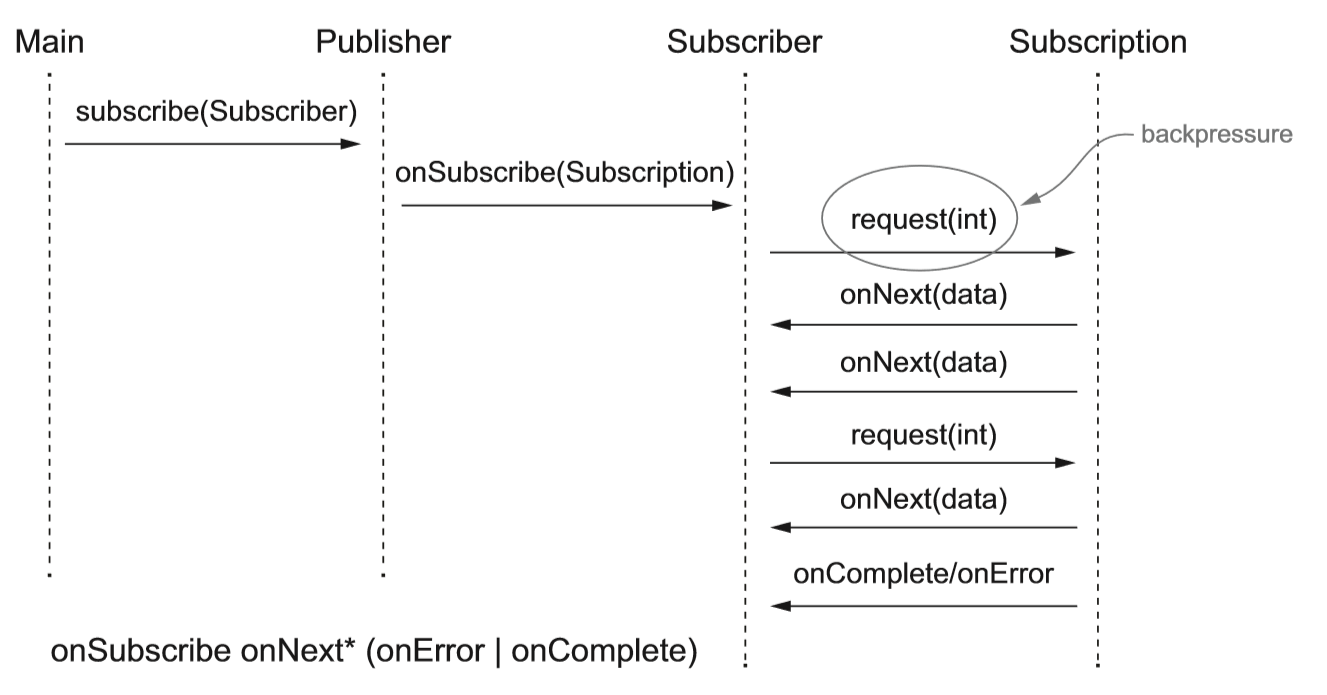
\includegraphics[width=\linewidth]{media/lifecycle}
    \label{lifecycle}
\end{figure} \footnote{vgl. Urma et al., S.424 \cite{buch:modern_java_in_action:kapitel17}}

Innerhalb des Mainthreads wird die Subscribe-Funktion, mit dem Subscriber als Argument, beim Publisher aufgerufen. Der Publisher ruft auf dem übergebenen Subscriber die Funktion onSubscribe auf, wobei die eine Subscription-Instanz des Publishers als Argument übergeben wird. Der Subscriber fordert eine bestimmte Anzahl an Datensätzen über die Request-Methode an. Die Subscription-Instanz ruft für die Anzahl an benötigten Daten die onNext-Methode des Subscribers auf. Dies geschieht, solange die Subscription keine onComplete- oder onError- Methode aufruft, denn damit ist die Subscription offiziell beendet. Die Request-Methode spielt hierbei eine besondere Rolle. Über diese lässt sich der Back-Pressure-Mechanismus realisieren, was im Kapitel \ref{subsubsec:backpressure} genauer betrachtet wird.

Anbieter wie z. B. RxJava, Reactor oder Akka implementieren die Reactive Streams Specifications.
So heißen die Reactive Streams in RxJava Flowable, in Akka-Streams Source und in Reactor Flux. Eine eingehendere Behandlung erfahren diese Begriffe in Kapitel \ref{chap:evaluierung}.
\subsection{Back Pressure}
\label{subsubsec:backpressure}
Unter Back Pressure versteht man die Regulierung des Datenflusses. In asynchronen Anwendungen kann es häufig zu einem Stau von Daten kommen, wenn beispielsweise der Publisher schneller Daten produziert als der Subscriber sie verarbeitet. Es gibt prinzipiell zwei Möglichkeiten, einen solchen Stau ohne Back Pressure zu vermeiden. \footnote{vgl. Grammes \& Schaal, 2015, S.44-45 \cite{web:artikel:javaspektrum} \label{grammesschaal}}
\begin{enumerate}
\item Der Subscriber reagiert auf den Stau und ordnet die Daten in eine Warteschlange ein. \footref{grammesschaal}
\item Der Publisher sendet kontinuierlich eine begrenzte Menge an Daten, sodass der Subscriber die Menge staufrei verarbeiten kann. \footref{grammesschaal}
\end{enumerate}

Bei Möglichkeit 1 kommen zwei Probleme auf. Wenn erstens die Größe der Warteschlange unbegrenzt ist, wird der Hauptspeicher irgendwann voll sein und einen Speicherüberlauf auslösen. Zweitens kann eine limitierte Größe der Warteschlange Datenverlust verursachen, wenn die Schlange voll ist.  \footref{grammesschaal}

Bei Möglichkeit 2 kann es passieren, dass die Leistung des Subscribers nicht vollständig ausgenutzt wird, wenn der Publisher zu wenig Daten produziert.  \footref{grammesschaal}

Back Pressure ermöglicht Überlastschutz über eine dynamische Anpassung des Datenflusses. Die Umsetzung gelingt über einen Push-Pull-Mechanismus. Push bezeichnet hier die Propagierung von Daten. Pull bezeichnet hingegen das Abholen von Daten. So wäre ein Push sinnvoll, wenn der Subscriber schneller als der Publisher ist, und ein Pull im gegenteiligen Fall.  \footref{grammesschaal}

Der Mechanismus des Back Pressure funktioniert so, dass zu Beginn davon ausgegangen wird, dass der Subscriber die Daten genauso schnell verarbeitet, wie der Publisher sie bereitstellt. Entsteht nun ein Stau, wechselt der Betrieb von Push zu Pull, was bedeutet, dass der Subscriber nun die Datenmenge anfordert, die er auch verarbeiten kann. So wird stets garantiert, dass zum einen kein Stau entsteht und zum anderen der Subscriber voll ausgelastet ist. \footref{grammesschaal}

\subsection{Streams oder Futures} \label{FutuProm}
Reactive Streams sind eine Spezifikation mit der Funktion, Informationen asynchron, nicht-blockierend und regulierend (Back Pressure) zu übertragen. Die Idee zur asynchronen, nicht-blockierenden Verarbeitung ist nicht neu und wurde bereits mit anderen Konzepten umgesetzt.

Futures sind Technologien die, wie Reactive Streams, reaktive Programmierung umsetzen.
Hierbei sind Futures ein Feature, das es bereits seit der Java-Version 5 gibt und im Package java.util.concurrent zu finden ist. Das Konzept dabei ist, eine Task asynchron durchzuführen, um blockierendes Warten zu vermeiden. Beim Aufruf wird direkt ein Future, also eine Referenz auf ein Ergebnis, geliefert, während die Task asynchron verarbeitet wird. Das Problem hierbei ist, dass einerseits der Status des Futures abgefragt werden muss, um zu erfahren, ob ein Ergebnis vorliegt. Andererseits kann es passieren, dass die asynchrone Task das Ergebnis nicht berechnet (Fehlerfall) und das Ergebnis somit nicht mehr verfügbar ist. Des Weiteren stellt es sich als schwer heraus, Ergebnisse von Futures aneinander zu reihen, da jedes Future wiederum auf Verfügbarkeit geprüft werden muss.\footnote{vgl. Urma et al., S.390 \cite{buch:modern_java_in_action:kapitel16} \label{futuresnpromisses}}

Seit der Java Version-8 wurden die CompletableFutures (java.util.concurrent), als konzeptuelle Erweiterung eingeführt. Die CompletableFutures können, im Gegensatz zu den Futures, verknüpft werden. Wenn eine asynchrone Operation von dem Ergebnis einer anderen abhängt, muss nun nicht-blockierend gewartet werden, bis das Ergebnis vorliegt, sondern kann direkt weitergeleitet werden. \footref{futuresnpromisses}

Sowohl Reactive Streams als auch Futures haben das Ziel, Tasks asynchron und nicht blockierend auszuführen. Der wesentliche Unterschied dieser Konzepte ist, dass Futures immer ein Element verarbeiten. So können zum Beispiel mehrere HTTP-Requests je in einem Future gemacht werden, während ein Stream keine theoretische Begrenzung hat. Des Weiteren sind Reactive Streams in der Lage, mittels Back Pressure Datenstaus zu vermeiden.

Die folgende Tabelle\footnote{vgl. Nurkiewicz und Christensen, Cardinality \cite{buch:reactive_programming_with_rxjava:kapitel1}} zeigt die Kardinalität von Technologien im asynchronen und synchronen Kontext: 

\begin{table}[H]
\centering
\caption{Szenarien und empfohlene Technologien}
\label{tab:scenariosandtech}
\begin{tabular}{
>{\columncolor[HTML]{C0C0C0}}l |c|c|}
\cline{2-3}
                                                        & \multicolumn{1}{l|}{\cellcolor[HTML]{00A99D}Ein Datensatz}                       & \multicolumn{1}{l|}{\cellcolor[HTML]{00A99D}Viele Datensätze}       \\ \hline
\multicolumn{1}{|l|}{\cellcolor[HTML]{00A99D}Synchron}  & Objekt                                                                           & \begin{tabular}[c]{@{}c@{}}Iterable,\\ Java Streams\end{tabular}    \\ \hline
\multicolumn{1}{|l|}{\cellcolor[HTML]{00A99D}Asynchron} & \begin{tabular}[c]{@{}c@{}}Callback, \\ Future,\\ CompletableFuture\end{tabular} & \begin{tabular}[c]{@{}c@{}}Reactive Stream,\\ Callback\end{tabular} \\ \hline
\end{tabular}
\end{table}

Für einfache synchrone Verarbeitungen mit einem Datensatz können simple Getter-Methoden genutzt werden, um das jeweilige Objekt zu erhalten. Falls viele Daten synchron verarbeitet werden müssen, eignen sich Iterable Typen respektive Streams. Im asynchronen Fall bieten sich Futures an. Selbst wenn es mehrere asynchrone Requests braucht, um eine Tasks zu verarbeiten, können dennoch CompleteableFutures verwendet werden. Bei vielen, asynchronen Datensätzen eignen sich vor allem die Reactive Streams.

\subsection{Collections API und Reactive Streams}
Der Begriff Stream kommt nicht nur in der reaktiven Programmierung vor, sondern auch in Java als native Bibliothek. Die Collections (in java.util.stream) unterstützen Streams als zusätzliche Abstraktionsebene, um deklarativ Informationen zu verarbeiten. Der so entstehende Vorteil ist, dass nun auf den imperativen Code von iterativen Schleifen verzichtet werden kann, was den Code allgemein wartbarer und verständlicher macht. Allerdings sind die Java Streams auf bestimmte Szenarien optimiert. Wie die Tabelle \ref{tab:scenariosandtech} zeigt, liegt die Stärke der Streams darin, Informationen synchron zu verarbeiten. Zwar ist es möglich, asynchrone Tasks zu verarbeiten, jedoch bietet die Streams-Api keine Möglichkeiten an die asynchronen Ergebnisse zu sortieren und zu synchronisieren. Vor allem in Situationen, in denen die asynchronen Tasks Latenzen haben oder undefinierte Zeitabstände vorweisen. Dies müsste manuell gelöst werden und würde die Komplexität des Codes stark erhöhen. Zudem gibt es keinen Mechanismus, der die Streams vor Überbelastung schützt.

Der Grund dafür, weshalb Java Streams in einen Kontext mit Reactive Streams gebracht werden, ist zum einen der Bezeichner Stream und zum anderen die deklarative Programmierung. Im späteren Teil dieser Thesis werden Implementierungen von Reactive Streams vorgestellt, die sich ähnlich deklarativ programmieren lassen wie die Java Streams. Die Möglichkeit der deklarativen Programmierung ist kein verpflichtendes Feature der Reactive Streams Specification und ist somit auch kein Teil von ihr.

Zusammengefasst liegt der Unterschied in dem Einsatzzweck: Java Streams sind für statische Daten geeignet, die einmal transformiert werden. Reactive Streams dagegen sind für dynamische, asynchrone Daten geeignet.

\subsection{Hot und Cold Streams}
\label{subsec:hotncold}
In vielen Implementierungen von Reactive Streams gibt es zwei Arten von Streams. Die Standard-Art ist der Cold Stream. Er reagiert mit dem Versenden der Daten, wenn eine Subscription erstellt wurde. Diese Art der Reaktion wird auch als lazy evaluation bezeichnet. Eine weitere Besonderheit ist, dass ein Cold Stream immer die gesamten Informationen für jede Subscription versendet. Ein Cold Stream ist somit nicht für Echtzeitdaten geeignet. Dieser Stream-Typ eignet sich besonders dann, wenn Informationen ein definiertes Ende haben, wie z. B. beim Inhalt einer Textdatei. \footnote{vgl. Davis, Hot and Cold \cite{buch:reactive_streams_in_java:kapitel3} \label{hot_and_cold}}

Ein Hot Stream dagegen versendet Daten unabhängig von Subscriptions. Das heißt, dass ein Subscriber immer die aktuellen Daten des Streams anstelle des gesamten Datensatzes empfängt. Hot Streams eignen sich dann, wenn die Informationen kein definiertes Ende haben, wie z. B. bei Twitter-Feeds. \footref{hot_and_cold}

\section{Reaktive Programmierung in reaktiven Systemen}
\label{sec:rpinrs}
Ein reaktives System ist ein Modell, das anhand von Qualitäten ein modernes, antwortbereites System beschreibt. Die reaktive Programmierung ist ein Paradigma, das Datenstrukturen in Streams asynchron, und nicht-blockierend verarbeitet. Beide Kontexte lassen sich miteinander vereinen, jedoch eignen sich die meisten reaktiven Bibliotheken nicht dafür, reaktive Systeme zu bauen.

Der Grund dafür ist die eventbasierte Kommunikation. Events haben keinen klaren Empfänger und stellen lediglich Fakten oder Signale dar. Die Widerstandsfähigkeit und Elastizität sind nicht ohne Weiteres realisierbar, da eine nachrichtenorientierte Kommunikation notwendig ist (siehe Kapitel \ref{sec:das_reaktive_manfiest}). Ein isolierter, ausgefallener Service muss adressierbar sein; falls er das nicht ist, weiß das System nicht, welcher Service wiederhergestellt werden soll.

Reaktive Programmiertechniken sind auf zeitlicher Ebene gut skalierbar, das heißt, sie sind für Nebenläufigkeit optimiert, während reaktive Systeme auf örtlicher Ebene skalierbar und daher verteilbar sind. Um ein reaktives System aus reaktiven Programmiertechnologien wie Streams und Futures zu bauen, benötigt es somit ergänzende Technologien wie z. B. Nachrichtenbusse, Fehlererkennungstechnologien (bspw. Hystrix) und Replikationstechniken (bspw. Docker).
\footnote{vgl. Benedikt Stemmildt \cite{web:youtube:going_reactive}; Bonér und Klang, S. 15 \cite{technischer_bericht:lightbend:rpvsrs}}

Ein prominentes Beispiel für die Verwendung von reaktiver Programmierung in reaktiven Systemen ist das Akka Toolkit. Die interne Verarbeitung der Daten und die Weiterleitung an Operatoren wird über eine Reactive-Streams-Implementierung realisiert. Das \href{https://akka.io/docs/}{Akka Toolkit} enthält noch weitere Technologien wie z. B. eine Implementierung des Aktorenmodells über die sich Nachrichten zwischen verschiedenen Diensten austauschen lassen. Es ist möglich, vollständige reaktive Systeme mit dem Toolkit zu bauen, da notwendige Technologien für die Streams bereits integriert sind. Anders als bei reinen Streams-Implementierungen wie RxJava und Reactor werden somit keine externen Abhängigkeiten (wie z. B. Message Bus und Verteilungssoftware) benötigt, was die \glslink{Homogen}{Homogenität} des gesamten Systems erhöht.

Es bietet sich an, die Dienste eines reaktiven Systems mit reaktiven Programmiertechniken zu bauen, denn auf der Anwendungsebene ist die reaktive Programmierung eine Alternative zu synchronen und blockierenden Programmen. In Kapitel \ref{chap:umsetzung} wird eine Anwendung reaktiv und klassisch implementiert, was im Anschluss in Performancetests miteinander verglichen wird.   
%
% Teil 2. Reaktive Programmierung in der Praxis
%
\chapter{Evaluierung}
\label{chap:evaluierung}
In diesem Kapitel werden reaktive Bibliotheken evaluiert und Frameworks betrachtet, die diese Bibliotheken nutzen. Es werden Kriterien evaluiert, die für das Unternehmen doubleSlash essentiell sind. Am Ende der Evaluierung werden die Kriterien und die Bewertung in einer gewichteten Evaluationsmatrix zusammengefasst. Die Gewichtung richtet sich nach den Prioritäten des Unternehmens. Die Matrix gilt als Ausgangspunkt für die Wahl der Bibliothek bei der Konzeption und Entwicklung der prototypischen Anwendung. 

\section{Wahl der zu betrachtenden Frameworks}
Konkret umfasst die Evaluierung drei reaktive Bibliotheken. Die Wahl der Bibliotheken basiert auf einer Umfrage der Seite \href{https://www.jaxcenter.de}{\textbf{jaxcenter.de}}. Die folgende Abbildung zeigt eine Umfrage zu Application Frameworks.

\begin{center}
\begin{figure}[H]
	\centering
	\caption{Jaxcenter Umfrage: Application Frameworks von 2016-2018}
  	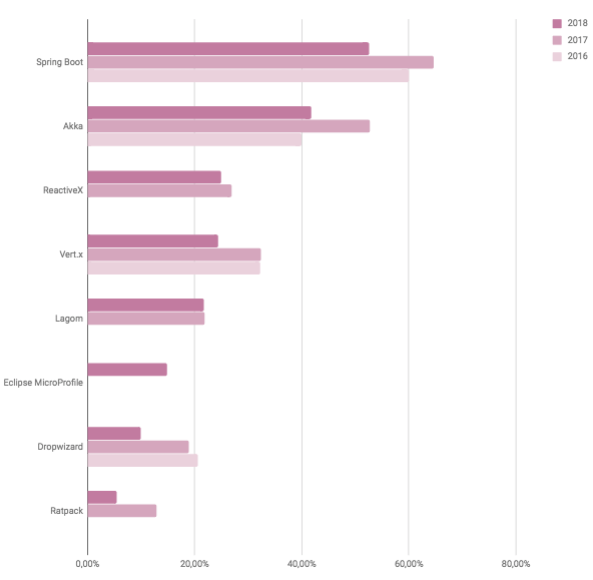
\includegraphics[width=.75\textwidth]{media/technologietrends.png}
	\label{jaxcenter:survey}
\end{figure}
\footnote{Schlosser und Richters, JAXenter-Survey: Application Frameworks - 2018, 2017, 2016 \cite{web:site:jaxcenter:trends}}
\end{center}

Gemäß den Technologietrends 2018 werden die Top 3 Spring-Boot, Akka und VertX betrachtet. Die korrespondierenden reaktiven Bibliotheken sind \hyperref[eval:rxjava]{\textbf{\nameref{eval:rxjava}}}, \hyperref[eval:reactor]{\textbf{\nameref{eval:reactor}}} und \hyperref[eval:akka-streams]{\textbf{\nameref{eval:akka-streams}}}. ReactiveX wird nicht als vollwertiges Framework wie Akka oder Spring betrachtet. Der Grund hierfür ist, dass ReactiveX sich selbst als API bezeichnet und nicht den technischen Umfang der anderen Frameworks aufweist. ReactiveX wird in vielen Programmiersprachen implementiert, weshalb die Verbreitung der ReactiveX API in Frontend (RxJs) und Backend (RxJava) stattfindet. Da Spring-Boot einen großen Umfang an Modulen besitzt, wird speziell das reaktive Web Framework WebFlux betrachtet.
\clearpage
Die folgende Abbildung zeigt einen Überblick über die bekanntesten reaktiven Frameworks/Toolkits und die dazugehörigen Bibliotheken.  

\begin{center}
\begin{figure}[H]
	\centering
    \caption{Überblick der reaktiven Bibliotheken und Frameworks}
    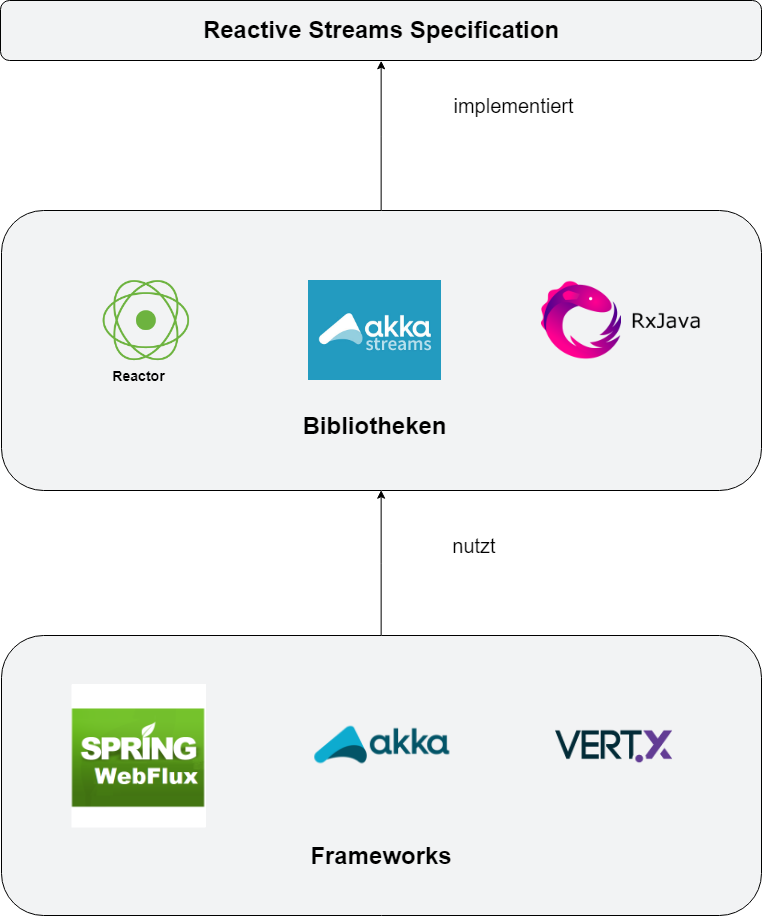
\includegraphics[width=.50\linewidth]{media/reactive_landscape}
    \label{benchmark}
\end{figure}
\end{center}

\section{Bibliotheken}
\subsection{Methodiken}
% Sonstige Befehle
\newcommand{\colorize}[1]{§\colorbox{yellow}{{#1}}§}
% Kriteriendefinition
\newcommand{\criteriaLizenz}{Lizenz und Kosten}
\newcommand{\criteriaSupport}{Support von Technologien}
\newcommand{\criteriaDoku}{Dokumentation}
\newcommand{\criteriaHandhabung}{Handhabung der Bibliothek}
\newcommand{\criteriaWeiterentwicklung}{Weiterentwicklung}
\newcommand{\criteriaVerbreitung}{Verbreitung}
Die Kriterien werden mittels der folgenden Methodiken evaluiert. Hierbei entsprechen die Kriterien den Anforderungen der Firma doubleSlash.

\begin{description}
\item \criteriaLizenz \\
Es ist zu prüfen ob die Bibliothek eine kommerzielle Nutzung zulässt und ob gegebenenfalls Kosten entstehen.
\item \criteriaDoku \\
Hierbei wird untersucht ob die Dokumentation umfassend, korrekt und aktuell ist.
\clearpage
\item \criteriaHandhabung \\
Es soll bewertet werden ob Programme kurz, prägnant und verständlich geschrieben werden können und ob eine falsche Bedienung verhindert bzw. erschwert wird.
\item \criteriaWeiterentwicklung \\
Es werden hierbei die Release-Daten untersucht und ermittelt ob Upgrades, Updates und Bugfixes regelmäßig erscheinen.
\item \criteriaVerbreitung \\
Die Ermittlung der Verbreitung wird zum einen über die Popularität auf GitHub verglichen und zum anderen über die Präsenz in der Entwickler-Community StackOverflow.
\end{description}

Die Bewertung der Kriterien beläuft sich auf ein Punkteschema. Jedes Kriterium wird zu Beginn mit zehn Punkten initialisiert. Für jedes negative Merkmal, dass bei der Betrachtung auffällt, gibt es Punktabzug. Die Menge an Punkten, die abzogen werden, richten sich nach der Schwere des Merkmals.

\subsection{RxJava}
\label{eval:rxjava}
RxJava steht für Reactive Extension (ReactiveX) Java. Die Reactive Extension wurde 2007 von Microsoft für .NET entwickelt. Die zunehmende Beliebtheit sorgte dafür, dass die API auch für andere Programmiersprachen implementiert wurde wie z. B. Javascipt, C\#, Scala, Swift, Clojure, C/C++, Python und viele mehr. Das Unternehmen Netflix hat RxJava implementiert und nutzt die Bibliothek für die Interprozesskommunikation und Verbindung verschiedener Services. In der Android Welt erfreut sich RxJava großer Beliebtheit. So nutzen Firmen wie SoundCloud, Square, NYT und Seatgeek die Bibliothek in ihren Apps.\footnote{vgl. Nurkiewicz und Christensen, Abs. 10 \cite{buch:reactive_programming_with_rxjava:foreword}}

RxJava gibt es in zwei Versionen. Version eins unterstützt nicht die Reactive Streams Specification und damit weder Back Pressure noch die Interkompatibilität mit anderen Bibliotheken. Version zwei dagegen ist eine Reimplementierung und unterstützt die Reactive Streams Specification. Im Rahmen dieser Thesis ist nur RxJava2 relevant. Die Bibliothek wird ab der Java Version 6 unterstützt.

Die Besonderheit von RxJava ist, dass die Daten der Publisher über Funktionen höherer Ordnung komponiert, gefiltert oder anderweitig transformiert werden können. Dieser funktionale Aspekt ermöglicht eine deklarative Programmierung. Unter dem Kriterium \href{handling:rxjava}{\criteriaHandhabung} wird gezeigt wie Nebenläufigkeit auf deklarative Art und Weise realisiert werden kann. 

Sowohl die Flow-Api als auch RxJava richten sich nach der Reactive Streams Specification. Folgende Tabelle zeigt die Flow-Typen und die RxJava Implementierungen: 

\begin{table}[H]
\centering
\caption{Flow Typen \& RxJava Typen (unvollständig)}
\begin{tabular}{|l|l|}
\hline
\rowcolor[HTML]{00A99D} 
Flow & RxJava \\ \hline
Publisher & Observable, Flowable \\ \hline
Subscriber & Observer, Single \\ \hline
Processor & Subject \\ \hline
Subscription & Disposable \\ \hline
\end{tabular}
\label{flow-api-to-rxjava}
\end{table}

Eine vollständige Liste der Typen in RxJava sind in der \href{http://reactivex.io/RxJava/javadoc/}{\textbf{Javadocs}} zu finden.

\subsubsection{\criteriaLizenz}
RxJava ist Open Source und besitzt die Apache-Lizenz 2.0 und ist daher für den kostenfreien, kommerziellen
Gebrauch zulässig. 

Da eine kommerzielle Nutzung erlaubt ist und keinerlei Kosten entstehen erhält RxJava zehn Punkte.

\begin{table}[H]
\begin{tabular}{|
>{\columncolor[HTML]{00A99D}}l |l|}
\hline
Punkte & 10 \\ \hline
\end{tabular}
\end{table}

\subsubsection{\criteriaDoku}
Auf der \href{https://reactivex.io}{\textbf{Homepage des Projekts}}\footnote{GitHub, ReactiveX Website \cite{web:site:reactivex}} befindet sich eine \href{http://reactivex.io/documentation}{\textbf{Referenzdokumentation}}, die die grundsätzlichen Typen und Mechanismen erklärt und illustriert. Diese Dokumentation soll primär die Kernkonzepte hinter ReactiveX vermitteln. Es handelt sich hierbei um eine allgemeine Referenz, die nicht programmiersprachenspezifisch ist.

Eine zweite Dokumentation gibt es auf GitHub in Form eines \href{https://github.com/ReactiveX/RxJava/wiki}{\textbf{Wiki}}\footnote{Github, ReactiveX Wiki \cite{web:github:reactivex:wiki}}. Das Wiki ist gut gegliedert und baut semantisch aufeinander auf. Für Java-Entwickler wird das Wiki für den Einstieg empfohlen, da alle relevanten Themen und weiterführende Informationen dort abgedeckt sind. Allerdings sind die Themen teils unvollständig dokumentiert.

Die \href{http://reactivex.io/RxJava/javadoc/}{\textbf{Javadocs}}\footnote{ReactiveX, Javadoc\cite{web:site:reactivex:javadoc}} lassen sich über das Wiki finden und sind auf dem aktuellen Stand des Releases. Die Dokumentation ist detailliert und enthält sämtliche Beschreibungen von Methoden, Klassen und Interfaces. Des Weiteren gibt es zu jeder Methode illustrierte Beispiele wie sie in der Praxis genutzt werden können.

Es gibt drei Punkte Abzug für die Unvollständigkeit der ReactiveX Referenzdokumentation. Die Überschriften im Wiki sind irreführend. Das Kapitel \href{https://github.com/ReactiveX/RxJava/wiki/Observable}{\textbf{reactive Types of RxJava}}\footnote{GitHub, ReactiveX Wiki \cite{web:github:reactivex:wiki:reactive_types}} suggeriert eine Auflistung der Typen, stattdessen wird auf die Referenzdokumentation verlinkt und der Observable Typ erklärt. 

\begin{table}[H]
\begin{tabular}{|
>{\columncolor[HTML]{00A99D}}l |l|}
\hline
Punkte & 7 \\ \hline
\end{tabular}
\end{table}

\subsubsection{\criteriaHandhabung}
\label{handling:rxjava}
Publisher und Subscriber können in RxJava kurz und prägnant ausgedrückt werden. Allerdings gibt es einige Aspekte, die eine falsche Benutzung ermöglichen. RxJava bietet eine Vielfalt an Typen für Publisher, Subscriber und Processor an. Das Problem ist, dass die große Menge an Typen eine umfangreichere Einarbeitung mit der Dokumentation benötigen. So wird in der Dokumentation als einziger reaktiver Typ das Observable genannt obwohl es weitaus mehr Typen für verschiedene Einsatzzwecke gibt. Das Flowable unterstützt Back Pressure während das Observable das nicht unterstützt. Die Verwechslung dieser Typen kann verheerend für das Programm sein.

Das folgende Listing zeigt ein Publisher (Flowable), welcher nacheinander die Events HELLO, WORLD und ! sendet. Der Subscriber (Observer) wird über zwei Methodenreferenzen und einer Lambda Funktion realisiert, welche implizit für die onNext, onError und onComplete Funktionen stehen. 

\begin{lstlisting}[language=java,  label={sourcecode:rxjava}, captionpos=t, caption={Synchron: RxJava Hello World}]
Flowable<String> flowable = Flowable.just("hello", "world", "!")
                                    .map(String::toUpperCase);
flowable.subscribe((next) -> 
				   System.out.println(Thread.currentThread.getName() 
				   						+ " " + next), // onNext
                   System.err::println,				   // onError
                   () -> System.out.println("done")); // onComplete
\end{lstlisting}
\clearpage

Das Programm erzeugt die folgende Ausgabe:

\begin{lstlisting}[language=bash,  label=ausgabe, captionpos=t, caption={Ausgabe vom synchronen Code}]
main HELLO
main WORLD
main !
done
\end{lstlisting}

Standardmäßig sind alle Publisher Typen (Observable, Flowable u. s. w.) synchron. Damit eine Subscription asynchron läuft, muss ein Threadpool respektiver Scheduler definiert werden, damit dieser auf einem Thread ausgelagert werden kann. Die Konfiguration hierfür ist allerdings simpel, da RxJava ein Set an Scheduler anbietet, die optimal auf das System abgestimmt sind. Das folgende Beispiel zeigt eine asynchrone Variante von \autoref{sourcecode:rxjava}.

\begin{lstlisting}[language=java,  label={sourcecode:rxjava:async}, captionpos=t, caption={Asynchron: RxJava Hello World (asynchron)}]
Scheduler scheduler = Schedulers.computation();
Disposable disposable = Flowable.just("hello", "world", "!")
.subscribeOn(scheduler) // Subscription auf einem Thread des Scheduler
.map(String::toUpperCase);
.subscribe(System.out::println,
     	   System.err::println,
           () -> System.out.println("done"));
while(!disposable.isDisposed()){}
\end{lstlisting}

Probleme in der Handhabung bei asynchroner Programmierung treten bei der Auswahl der Funktionen auf. RxJava bietet zwei Funktionen zur asynchronen Ausführung an. Zum einen subscribeOn (wie in \autoref{sourcecode:rxjava:async}) und zum anderen observeOn. Mit subscribeOn kann definiert werden mit welchem Scheduler die Subscription ausgelagert wird. Das heißt, dass alle Elemente auf einen anderen Thread geschickt werden und dort vom Subscriber über onNext, onError u. s. w. verarbeitet werden.

Die Funktion observeOn dagegen, definiert, auf welchen Thread einzelne Operationen ausgeführt werden können. Das heißt, dass alle Funktionen, die nach dem Aufruf von observeOn aufgerufen werden, auf einem anderen Thread laufen.

Das folgende Listing zeigt den Ausschnitt einer asynchronen Variante mit subscribeOn und observeOn. Über die Funktion doOnNext können schrittweise die Elemente ausgegeben werden. In diesem Beispiel wird der aktuelle Thread und das dazugehörige Element ausgegeben.
\clearpage
\begin{lstlisting}[language=java,  label={sourcecode:rxjava:async:debug}, captionpos=t, caption={RxJava Hello World debug}]
Flowable.just("hello", "world", "!")
.map(String::toUpperCase)
.doOnNext((element) -> System.out.println(Thread.currentThread()
										  .getName()+ " " + element))
.subscribeOn(scheduler)
.observeOn(scheduler) // Nachfolgende Funktionen auf anderem Thread des Schedulers
.filter(word -> word.length() > 1)
.subscribe((next) -> System.out.println(Thread.currentThread()
										      .getName()+" "+next),
                  System.err::println,
	              () -> System.out.println("done"));
\end{lstlisting}

Aufgrund dessen, dass das Programm multithreaded läuft, ist das nachfolgende Listing ein Beispiel:

\begin{lstlisting}[language=java,  label={sourcecode:rxjava:async:debug:ausgabe}, captionpos=t, caption={Ausgabe}]
RxComputationThreadPool-2 HELLO
RxComputationThreadPool-2 WORLD
RxComputationThreadPool-2 !
RxComputationThreadPool-1 HELLO
RxComputationThreadPool-1 WORLD
done
\end{lstlisting}

Die Ausgabe zeigt, dass die Verarbeitung des Flowables nicht auf dem Main Thread stattfindet, sondern auf dem RxComputationThreadPool-2 Thread. Die Funktionen, die nach dem Aufruf von observeOn folgen, werden auf dem RxComputationThreadPool-1 Thread ausgeführt wie z. B. der Aufruf der Filterfunktion. Das bedeutet, dass es entscheidend ist, wann die observeOn Funktion aufgerufen wird. Je nachdem wann die Funktion aufgerufen wird, werden alle folgenden Funktionen auf einem anderen Thread ausgelagert. Bei subscribeOn spielt die Reihenfolge keine Rolle, da die Subscription asynchron läuft und somit implizit der gesamte Stream mit allen Funktionen verlagert wird.

Bei der asynchronen Programmierung kann es schnell zur falschen Benutzung kommen, wenn die Anwendungsfälle der Funktionen nicht klar sind. Die freie Benutzung der Threadpools und Scheduler soll eine maximale Transparenz und eine freie Auswahl bezüglich Scheduler bieten. Für Anfänger wirkt das nicht intuitiv und verleitet zur falschen Benutzung.

Insgesamt gibt es zwei Punkte Abzug für die große Anzahl an Typen, die die API unübersichtlichen machen und eine falsche Benutzung der Typen ermöglichen. Des Weiteren gibt es noch zwei Punkte Abzug für das unkonventionelle Multithreading. Die deklarative Art erleichtert zwar die nebenläufige Programmierung, allerdings muss der Entwickler aufpassen in welchen Kontext, welche Funktion verwendet wird. Ein zu früh platzierter observeOn-Aufruf verlagert zu viele Operatoren auf einen anderen Thread und kann ihn überlasten. In der Praxis wird die observeOn-Funktion hinter der Subscribefunktion aufgerufen. Somit kann der Entwickler bestimmen, auf welchem Thread der Subscriber die Events verarbeitet. 
        
\begin{table}[H]
\begin{tabular}{|
>{\columncolor[HTML]{00A99D}}l |l|}
\hline
Punkte & 6 \\ \hline
\end{tabular}
\end{table}

\subsubsection{\criteriaWeiterentwicklung}
Um die Weiterentwicklung einer Bibliothek qualitativ zu bewerten werden Statistiken von dem Repository auf GitHub verglichen.

Der folgende Ausschnitt zeigt die Release-Zyklen des Projekts.
\begin{table}[H]
\caption{Ausschnitt aus den Releases}
\centering
\begin{tabular}{|l|l|}
\hline
\rowcolor[HTML]{00A99D} 
Version & Datum      \\ \hline
2.2.4   & 23.11.2018 \\ \hline
2.2.3   & 23.10.2018 \\ \hline
2.2.2   & 06.09.2018 \\ \hline
2.2.1   & 23.08.2018 \\ \hline
2.2.0   & 29.07.2018 \\ \hline
2.1.17  & 23.07.2018 \\ \hline
\end{tabular}
\end{table}

Es wird jeden Monat mindestens eine neue Version veröffentlicht. Die Nebenversionen werden hingegen unterschiedlich veröffentlicht. Die monatlichen Releases enthalten Bugfixes, Dokumentation und API-Erweiterungen. 

Insgesamt wird die Bibliothek aktiv weiterentwickelt und erhält regelmäßige Updates. Das Kriterium ist vollständig erfüllt.

\begin{table}[H]
\begin{tabular}{|
>{\columncolor[HTML]{00A99D}}l |l|}
\hline
Punkte & 10 \\ \hline
\end{tabular}
\end{table}

\subsubsection{\criteriaVerbreitung}
Um die Verbreitung einer Bibliothek zu messen werden verschiedene Metriken verwendet. Zum einen wird die Anzahl an getaggten Fragen auf StackOverflow verglichen. Die Anzahl sagt aus wie häufig Fragen bezüglich der Bibliothek gestellt werden. Die statistischen Werte auf GitHub sagen aus wie viele Personen sich für die Bibliothek interessieren. 

Die folgende Abbildung zeigt wie die Daten auf StackOverflow erhoben werden:
\begin{center}
\centering
\begin{figure}[H]
\caption{Erhebung der Daten auf StackOverflow}
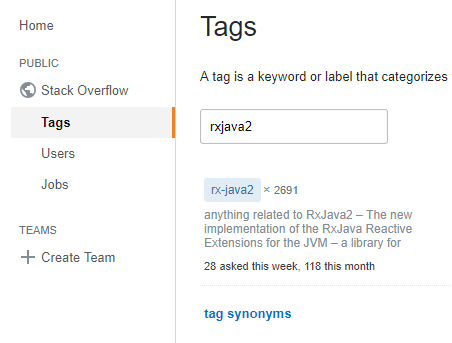
\includegraphics[width=.5\textwidth]{media/stackoverflow_rxjava}
\label{stackoverflow:rxjava}
\end{figure}
\end{center}

Die folgende Tabelle zeigt einen Schnappschuss aus StackOverflow\footnote{Quelle: \cite{web:site:stackoverflow:rxjava}, \cite{web:site:stackoverflow:akka}, \cite{web:site:stackoverflow:akka}}, wobei die Anzahl aktiv diskutierter Fragen im Kontext der jeweiligen Bibliothek betrachtet wird:

\begin{table}[H]
\centering
\caption{Schnappschuss aktiv diskutierter Fragen (Stand 03.12.2018)}
\begin{tabular}{|l|l|}
\hline
\rowcolor[HTML]{00A99D} 
Bibliothek   & Diskutierte Fragen \\ \hline
RxJava       & 2628   \\ \hline
Reactor     & 762    \\ \hline
Akka Streams & 1131   \\ \hline
\end{tabular}
\label{stackoverflow_snapshot}
\end{table}

Es zeigt sich, dass RxJava die am meisten diskutierte Bibliothek auf StackOverflow ist.

Die zweite Metrik stützt sich auf statistische Daten der Open Source Plattform GitHub. Hierbei wird die Anzahl an öffentlichen Repositories \footnote{Github Quelle zu den Repositories \cite{web:site:github:count:repo:rxjava} \cite{web:site:github:count:repo:reactor}, \cite{web:site:github:count:repo:akka}} sowie die Anzahl an Stars, die die Bibliothek hat, betrachtet. Die Stars eines Projektes sind als Wertschätzung für die Maintainer zu verstehen. GitHub nutzt diese Zahl zum globalen Ranking von Projekten.\footnote{vgl. GitHub, About Stars \cite{web:site:github:about_stars}} Damit wird die Popularität und Bekanntheit innerhalb der Community verstanden.

\begin{table}[H]
\caption{GitHub Statistik}
\centering
\begin{tabular}{l|l|l|l|}
\cline{2-4}
              & \cellcolor[HTML]{00A99D}RxJava & \cellcolor[HTML]{00A99D}Reactor & \cellcolor[HTML]{00A99D}Akka Stream \\ \hline
\multicolumn{1}{|l|}{\cellcolor[HTML]{00A99D}Repositories}  & 9005                          & 876                             & 836                                \\ \hline
\multicolumn{1}{|l|}{\cellcolor[HTML]{00A99D}Projekt Stars} & 36772                         & 2761                            & 9331                               \\ \hline
\multicolumn{1}{|l|}{\cellcolor[HTML]{00A99D}Ranking}		  & \href{https://gitstar-ranking.com/ReactiveX/RxJava}{48}							   & \href{https://gitstar-ranking.com/reactor/reactor}{3743}							 & \href{https://gitstar-ranking.com/akka/akka}{955}								   \\ \hline
\end{tabular}
\label{github:statistic}
\end{table}
\footnote{Da die Akka-Streams Bibliothek in Scala programmiert ist, wird die Anzahl Repositories unter der Sprache Scala betrachtet.}

Das Ranking wird über die Seite \href{www.gitstar-ranking.com}{www.gitstar-ranking.com}\footnote{Gitstar Quelle zum Ranking: \cite{web:site:gitstar-ranking:rxjava}, \cite{web:site:gitstar-ranking:reactor}, \cite{web:site:gitstar-ranking:akka}} ermittelt. 

Die Auswertung zeigt, dass RxJava mit über 8000 Repositories am häufigsten in Teilen von Projekten vorkommt. Des Weiteren hat die Bibliothek selbst über 36600 Stars, was unter den weltweiten Projekten (ca. 28 Millionen öffentliche Repositories)\footnote{Wikipedia \cite{web:wiki:github}} den 48. Platz belegt und somit weit vor Reactor und Akka steht.

Insgesamt ist RxJava auf StackOverflow die am meisten diskutierte Bibliothek. Auf GitHub werden statistisch mehr Projekte mit RxJava erstellt, das Repository der Bibliothek hat weitaus mehr Stars und belegt unter den Open Source Projekten den höchsten Platz. RxJava ist somit die am weitesten verbreitetste reaktive Bibliothek. Es gibt somit keinen Punktabzug.

\begin{table}[H]
\begin{tabular}{|
>{\columncolor[HTML]{00A99D}}l |l|}
\hline
Punkte & 10 \\ \hline
\end{tabular}
\end{table}

\subsection{Reactor}
\label{eval:reactor}
Die Bibliothek Reactor wird von Pivotal \& Spring vertrieben und implementiert die Reactive Streams Specification. Reactor wurde in Kollaboration mit Spring für das Webflux Framework entwickelt und ist ein Kernbestandteil davon. Aufgrund dessen das WebFlux relativ neu ist, unterstützt Reactor Java ab Version 8. Die folgende Tabelle zeigt eine Gegenüberstellung der Typen.

\begin{table}[H]
\caption{Flow \& Reactor (unvollständig)}
\centering
\begin{tabular}{|l|l|}
\hline
\rowcolor[HTML]{00A99D} 
Flow         & Reactor       \\ \hline
Publisher    & Flux, Mono    \\ \hline
Subscriber   & Subscriber    \\ \hline
Processor    & FluxProcessor \\ \hline
Subscription & Disposable    \\ \hline
\end{tabular}
\label{flow_to_reactor}
\end{table}

Weitere Typen und nähere Beschreibungen sind in der \href{https://projectreactor.io/docs/core/release/api/}{\textbf{Javadoc}}\footnote{Reactor, Javadoc \cite{web:site:reactor:javadoc} \label{lbl:reactor:javadoc}} zu finden.

\subsubsection{\criteriaLizenz}
Reactor ist Open Source und besitzt die Apache-Lizenz 2.0 und ist daher für den kostenfreien, kommerziellen
Gebrauch zulässig. 

Da eine kommerzielle Nutzung erlaubt ist und keinerlei Kosten entstehen, erhält Reactor keinen Abzug.
\begin{table}[H]
\begin{tabular}{|
>{\columncolor[HTML]{00A99D}}l |l|}
\hline
Punkte & 10 \\ \hline
\end{tabular}
\end{table}

\subsubsection{\criteriaDoku}
Reactor besitzt eine umfangreiche \href{https://projectreactor.io/docs/core/release/reference/}{Referenzdokumentation}\footnote{Reactor, Referenz \cite{web:site:reactor:reference}} und eine \href{https://projectreactor.io/docs/core/release/api/}{Javadoc}\footref{lbl:reactor:javadoc}. Die Referenz deckt grundlegende Fragen zur reaktiven Programmierung ab und führt in die Thematik ein. Des Weiteren wird auf die Installation, Kernkonzepte und weiter führende Themen eingegangen. Insgesamt ist die Referenz informativ und deckt alle Fragen für Neu- und Quereinsteiger ab.

Die Javadocs sind auf dem aktuellen Stand des Releases. Es werden in den Javadocs ebenfalls Illustrationen für die Funktionen verwendet.

Aufgrunddessen, dass Reactor eine geringe Anzahl an Typen hat, wirkt die API schlank und übersichtlich und ermöglicht schnelle Designentscheidungen im Bezug auf die Wahl der richtigen Typen.

Insgesamt ist die Referenzdokumentation als auch die Javadocs sehr übersichtlich und klar strukturiert. Die Reactor Bibliothek erhält die volle Punktzahl.

\begin{table}[H]
\begin{tabular}{|
>{\columncolor[HTML]{00A99D}}l |l|}
\hline
Punkte & 10 \\ \hline
\end{tabular}
\end{table}

\subsubsection{\criteriaHandhabung}
In Reactor können Publisher und Subscriber kurz und prägnant geschrieben werden. Die API ist der von RxJava sehr ähnlich. Der wesentliche Unterschied liegt darin, dass Reactor weniger Typen anbietet. Im Gegensatz zu RxJava bietet Reactor zwei Publisher-Typen an: Mono und Flux. Beide unterstützen standardmäßig das Back Pressure. Mono und Flux stehen jeweils für eine bestimmte Kardinalität. Mono verarbeitet Events in Anzahl 0 bis 1 während Flux 0 bis n verarbeitet. 

Das folgende Beispiel zeigt einen Flux, dass nacheinander HELLO, WORLD und ! emittiert.

\begin{lstlisting}[language=java, captionpos=t, caption={Synchron: Reactor Hello World!}, breaklines=true]
Flux<String> flux = Flux.just("hello", "world", "!")
                		.map(String::toUpperCase);
flux.subscribe((next)->System.out.println(Thread.getCurrentThread.getName()+" "+next),
               System.err::println,
               ()->System.out.println("done"));
\end{lstlisting}

Der Quellcode ist, bis auf die Namen, identisch mit dem Quellcode aus \ref{sourcecode:rxjava} in RxJava. 
Die Ausgabe ist äquivalent zur Ausgabe in \ref{ausgabe}. 

Bei der asynchronen Ausführung gibt es nur namentliche Unterschiede. Von der Menge des Codes und von der Semantik ist die Reactorimplementierung identisch mit der asynchronen Variante von RxJava in \ref{sourcecode:rxjava:async}. 
\clearpage
\begin{lstlisting}[language=java,  captionpos=t, caption={Asynchron: Reactor Hello World!}, breaklines=true]
Scheduler scheduler = Schedulers.parallel();
Disposable disposable = Flux.just("hello", "world", "!")
                            .map(String::toUpperCase)
                            .subscribeOn(scheduler)
                            .subscribe(
        	                    System.out::println,
                                System.err::println,
                                () -> System.out.println("done"));
while(!disposable.isDisposed()){}
\end{lstlisting}

Reactor hat, wie RxJava, ebenfalls zwei Methoden zur asynchronen Ausführung. Zum einen subscribeOn, welches dem subscribeOn in RxJava entspricht und zum anderen publishOn, was dem observeOn entspricht. Das Problem hierbei ist, wie bei RxJava, dass die Funktionen falsch benutzt werden können. \footnote{vgl. Kapitel \ref{handling:rxjava}} 

Zusammengefasst ist es relativ schwierig die Bibliothek falsch zu bedienen. Die schlanke API lässt es kaum zu, falsche Typen zu verwenden. Lediglich bei der asynchronen Programmierung können dieselben Probleme auftreten wie bei RxJava, weshalb die Bibliothek diesbezüglich zwei Punkte abgezogen bekommt.

\begin{table}[H]
\begin{tabular}{|
>{\columncolor[HTML]{00A99D}}l |l|}
\hline
Punkte & 8 \\ \hline
\end{tabular}
\end{table}

\subsubsection{\criteriaWeiterentwicklung}
Das Reactor Projekt wird in GitHub unter drei Versionen vertrieben. Version eins und zwei sind veraltet und werden nicht mehr aktiv weiterentwickelt. Für Version drei nutzen die Maintainer ein dreigleisiges Versionsschema. Die folgende Tabelle die Versionierung von Reactor3.

\begin{table}[H]
\caption{Versionsgleise und Versionsnummern}
\centering
\begin{tabular}{|l|l|}
\hline
\rowcolor[HTML]{00A99D} 
Versions-Gleis & Versionsnummer \\ \hline
Aluminium      & 3.0.x          \\ \hline
Bismuth        & 3.1.x          \\ \hline
Californium    & 3.2.x          \\ \hline
\end{tabular}
\end{table}

Die Versionsnummern entsprechen der Version der reactor-core Bibliothek. Die Reactor Bibliothek enthält zusätzlich zur Core Bibliothek noch einen Http und TCP Server (Reactor Netty) und Reactor Addons für die Interoperabilität zwischen verschiedenen Bibliotheken. Somit besteht die Reactor Bibliothek aus drei Unterbibliotheken.

Die Aluminium Version wurde seit zwei Jahren nicht mehr aktualisiert. Die Bismuth Version wird noch aktiv weiterentwickelt und erhält regelmäßig Updates. Die Hauptunterschiede zwischen den Nebenversionen sind Features und Namensänderungen. Die Versionsgleise sind somit nicht miteinander kompatibel.

\begin{table}[H]
\caption{Ausschnitt der Releases}
\centering
\begin{tabular}{|l|l|}
\hline
\rowcolor[HTML]{00A99D} 
Version & Datum      \\ \hline
3.2.3   & 23.11.2018 \\ \hline
3.2.2   & 31.10.2018 \\ \hline
3.2.1   & 10.10.2018 \\ \hline
3.2.0   & 21.09.2018 \\ \hline
3.1.0   & 25.09.2017 \\ \hline
3.0.0   & 23.08.2016 \\ \hline
\end{tabular}
\end{table}

Die Nebenversionen (Versionsgleise) werden kontinuierlich in Jahreszyklen veröffentlicht. Revisionen werden monatlich veröffentlicht.

Insgesamt wird die Bibliothek aktiv weiterentwickelt und erhält regelmäßig Updates. Das Kriterium ist vollständig erfüllt.

\begin{table}[H]
\begin{tabular}{|
>{\columncolor[HTML]{00A99D}}l |l|}
\hline
Punkte & 10 \\ \hline
\end{tabular}
\end{table}

\subsubsection{\criteriaVerbreitung}
\begin{table}[H]
\caption{GitHub Statistik}
\centering
\begin{tabular}{l|l|l|l|}
\cline{2-4}
              & \cellcolor[HTML]{00A99D}RxJava & \cellcolor[HTML]{00A99D}Reactor & \cellcolor[HTML]{00A99D}Akka Stream \\ \hline
\multicolumn{1}{|l|}{\cellcolor[HTML]{00A99D}Repositories}  & 9005                          & 876                             & 836                                \\ \hline
\multicolumn{1}{|l|}{\cellcolor[HTML]{00A99D}Projekt Stars} & 36772                         & 2761                            & 9331                               \\ \hline
\multicolumn{1}{|l|}{\cellcolor[HTML]{00A99D}Ranking}		  & \href{https://gitstar-ranking.com/ReactiveX/RxJava}{48}							   & \href{https://gitstar-ranking.com/reactor/reactor}{3743}							 & \href{https://gitstar-ranking.com/akka/akka}{955}								   \\ \hline
\end{tabular}
\label{github:statistic:reactor}
\end{table}

\begin{table}[H]
\centering
\caption{Schnappschuss aktiv diskutierter Fragen}
\begin{tabular}{|l|l|}
\hline
\rowcolor[HTML]{00A99D} 
Bibliothek   & Diskutierte Fragen \\ \hline
RxJava       & 2628   \\ \hline
Reactor     & 762    \\ \hline
Akka Streams & 1131   \\ \hline
\end{tabular}
\label{stackoverflow_snapshot:reactor}
\end{table}

Gemäß der Tabelle \ref{github:statistic:reactor} erreicht Reactor die niedrigste Platzierung der drei Bibliotheken. Auf StackOverflow erreicht Reactor ebenfalls eine geringere Anzahl an Fragen pro Tag, wie in \ref{stackoverflow_snapshot:reactor} zu sehen ist. Die Auswertung sagt nicht aus, dass die Bibliothek nicht verbreitet ist sondern, dass sie weniger verbreitet ist als Akka-Streams oder RxJava.

Da Reactor Kernbestandteil von Webflux ist, wird es implizit in allen Spring Webflux Anwendungen genutzt. Weiterhin bietet Spring zusätzlich eine Vielzahl an Integration an wie z. B. in Spring Data und Spring Security.

Allerdings ist Reactor eine Bibliothek, die stark an Popularität zunimmt. Der Chefentwickler von RxJava Dave Karnok antwortet auf die Frage, in welchen Situationen Reactor oder RxJava genutzt werden soll mit folgendem Satz: 
\begin{quote}
Use Reactor 3 if you are allowed to use Java 8+, use RxJava 2 if you are stuck on Java 6+ or need your functions to throw checked exceptions. \footnote{David Karnok, Twitter Posting \cite{web:site:twitter:feed:dave_karnok}}
\end{quote}

Insgesamt ist die Reactor Bibliothek, die am wenigsten verbreitete. Ausgehend von drei Plätzen, werden für jeden Platz 3 Punkte vergeben. Der Erste erhält 4 Punkte dem zweiten gegenüber. Somit bekommt die Bibliothek 7 Punkte Abzug.

\begin{table}[H]
\begin{tabular}{|
>{\columncolor[HTML]{00A99D}}l |l|}
\hline
Punkte & 3 \\ \hline
\end{tabular}
\end{table}

\subsection{Akka-Streams}
\label{eval:akka-streams}
\label{intro:akka-streams}
Akka-Streams ist die Stream Bibliothek des Akka Toolkits und wird ab der Javaversion 8 unterstützt. Die Besonderheit der Bibliothek ist, dass die Flow Typen nicht direkt als Schnittstelle angeboten werden sondern ausschließlich über die Implementierungen zur Verfügung stehen. Das heißt, dass die Publisher, Subscriber u. s. w. nicht direkt zugänglich sind. Die Entwickler der Akka-Streams betrachten die Reactive Streams Specification nicht als End-User API sondern als SPI (Service Provider Interface). \footnote{vgl. Lightbend, Inc., Relationship with Reactive Streams, 2018 \cite{web:akka:def:streams}} Das heißt, dass die Schnittstelle ausschließlich für die Entwickler freigegeben wird und nicht für die Nutzer der Bibliothek. Die schwer zu implementierenden Interfaces sollen somit verborgen bleiben und über einfachere Abstraktionen bedienbar sein. Bibliotheken wie RxJava und Reactor bieten auch Abstraktionen zu Publishern und Subscriber an (Observable, Flux), allerdings kann der Entwickler auch eigene Publisher implementieren.

Die folgende Tabelle stellt die Flow Typen den Akka-Streams Typen gegenüber: 

\begin{table}[H]
\caption{Flow \& Akka-Streams}
\centering
\begin{tabular}{|l|l|}
\hline
\rowcolor[HTML]{00A99D} 
Flow         & Akka-Streams \\ \hline
Publisher    & Source       \\ \hline
Subscriber   & Sink         \\ \hline
Processor    & Flow         \\ \hline
Subscription & Materializer \\ \hline
\end{tabular}
\label{flow_to_akka}
\end{table}
\clearpage
Ein Typischer Akka Stream sieht wie folgt aus:

\begin{center}
\begin{figure}[H]
\centering
\caption{Akka-Stream Beispiel}
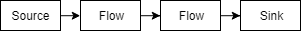
\includegraphics[width=.75\textwidth]{media/akka-stream}
\label{fig:akka-stream}
\end{figure}
\end{center}

Eine oder mehrere Sources definieren die Datenquelle und können Nachrichten aus primitiven Datentypen, Collections und Arrays erzeugen. Am Ende der Verarbeitungskette befinden sich eine oder mehrere Sinks, welche die ankommenden Daten verarbeiten. Zwischen Source und Sink können Flows platziert werden, die weitere Verarbeitungsschritte umsetzen. Der Materializer alloziert die notwendigen Ressourcen der Prozessschritte und führt diese aus. Diese Art der Verarbeitung ermöglicht eine Entkoppelung der Verarbeitungsschritte und damit eine Wiederverwendung. \footnote{vgl. Lightbend Inc., Core Concepts \cite{web:akka:docs:streams_flows_and_basics}\label{akka:concept}}

In Akka-Streams werden Verarbeitungsketten von Source, Flows und Sinks als Graphen bezeichnet. Ein Graph beschreibt die Topologie der Verarbeitungsschritte. Der Stream aus \autoref{fig:akka-stream} ist ein trivialer Graph. Komplexe Graphen können auch aus mehreren Eingabe- und Ausgabekanälen bestehen. 

\subsubsection{\criteriaLizenz}
Akka-Stream ist Open Source und besitzt die Apache-Lizenz 2.0 und ist daher für den kostenfreien, kommerziellen
Gebrauch zulässig.

Da eine kommerzielle Nutzung erlaubt ist und keinerlei Kosten entstehen erhält Akka-Stream 10 Punkte.
\begin{table}[H]
\begin{tabular}{|
>{\columncolor[HTML]{00A99D}}l |l|}
\hline
Punkte & 10 \\ \hline
\end{tabular}
\end{table}

\subsubsection{\criteriaDoku}
Akka bietet eine übersichtliche \href{https://akka.io/docs/}{\textbf{Referenzdokumentation}}\footnote{Lightbend, Docs \cite{web:akka:docs}} für alle Module an. Hierbei können Code-Beispiele wahlweise in Scala oder Java betrachtet werden. Module, die Teil von Akka sind, entsprechen immer der Repository Version. Die aktuelle Akka Version ist 2.5.19 (Stand 10.12.2018). Die \href{https://doc.akka.io/docs/akka/current/stream/index.html?language=java}{\textbf{Akka-Stream Referenz}}\footnote{Lightbend, Referenz \cite{web:akka:docs:streams}} bietet eine gegliederte Übersicht über alle Teilaspekte der Streams an wie z. B. grundlegende Datentypen wie Source und Sink, IO Verarbeitung, Graphen u. v. m. .

Die \href{https://doc.akka.io/japi/akka/current/index.html?akka/stream/package-summary.html&_ga=2.134194124.394401883.1544449904-1435486093.1536821504}{\textbf{Javadocs}}\footnote{Lightbend, Javadoc \cite{web:akka:javadoc}} sind auf dem aktuellen Stand des Releases. Ein Problem der Dokumentation ist, dass sie nicht nur die Streams enthält, sondern alle restlichen Akka Module wie z. B. Actor, Cluster und Persistence. Das hat zur Folge, dass die Doku sehr umfangreich und unübersichtlich ist. Die Beschreibung ist detailliert und teilweise mit Code-Beispielen versehen.

Insgesamt sind die Javadocs gut und hilfreich, allerdings werden einige Funktionen wie z. B. fold und scan rein textuell erklärt und weder mit Code-Beispielen noch mit Diagrammen vereinfacht dargestellt. Hierfür gibt es 2 Punkte Abzug. Die folgende Abbildung zeigt ein Beispiel der schlecht dokumentierten Funktion scan und fold:

\begin{center}
\begin{figure}[H]
\centering
\caption{Ausschnitt aus der Dokumentation der Funktionen scan und fold}
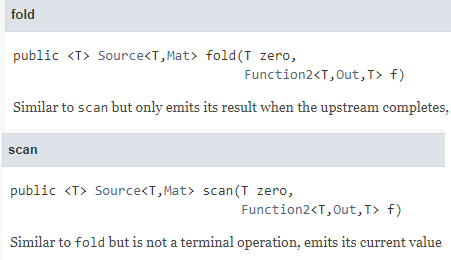
\includegraphics[width=.75\textwidth]{media/genius}
\label{fig:akka-stream:javadoc}
\end{figure}
\end{center}

Die Referenzdokumentation hat relativ schwer nachvollziehbare Codebeispiele, die das Wesentliche kompliziert darstellen. Hierfür gibt es drei Punkte Abzug, da für das Kapitel \href{https://doc.akka.io/docs/akka/current/stream/stream-graphs.html}{Working with Graphs} einiges an Recherche gemacht werden muss, die nicht in den Grundlagen erklärt werden.

\begin{table}[H]
\begin{tabular}{|
>{\columncolor[HTML]{00A99D}}l |l|}
\hline
Punkte & 5 \\ \hline
\end{tabular}
\end{table}

\subsubsection{\criteriaHandhabung}
Publisher und Subscriber können bedingt kurz und prägnant ausgedrückt werden. Grundsätzlich unterscheidet sich die Akka-Stream Bibliothek sehr stark von RxJava und Reactor. Das Vokabular rund um Akka-Stream ist deutlich größer als das von RxJava oder Reactor. Der Code sieht unübersichtlich aus und enthält viele Typen. Allerdings entfällt die Unübersichtlichkeit und der Boilerplate Code, wenn Scala statt Java verwendet wird. Akka-Stream ist eine Bibliothek, die in erster Linie in Scala entwickelt wurde und die Eigenschaften dieser Sprache optimal nutzt. In Java wirkt der Code deutlich komplexer, was auch die Handhabung beeinträchtigt.

Das folgende Beispiel demonstriert das (asynchrone) Emittieren von HELLO, WORLD und !.

\begin{lstlisting}[language=java,  label={sourcecode:akka}, captionpos=t, caption={Akka Streams Hello World}, breaklines=false]
ActorSystem actorsystem = ActorSystem.create();
Materializer materializer = ActorMaterializer.create(system);
Source<String, NotUsed> source = Source
								 .from(Arrays.asList("hello",
								 					 "world",
								 					 "!"))
                                 .map(String::toUpperCase);
Sink<String, CompletionStage<Done>> sink = Sink
										   .foreach(System.out::println);
CompletionStage<Done> done = source.runWith(sink, materializer);
done.thenRun(() -> {
	System.out.println("done");
    actorsystem.terminate();});
\end{lstlisting}

Die Ausgabe ist äquivalent zur Ausgabe in \autoref{ausgabe}.

In Akka erfolgt die Kommunikation zwischen asynchronen Endpunkten immer über Nachrichten mehrerer Aktoren. Damit ein Programm die Aktoren nutzen kann, benötigt es eine Laufzeitumgebung für die Aktoren, dem Aktorensystem (Zeile 1). Wie in \autoref{intro:akka-streams} bereits beschrieben, werden Definition und Ausführung getrennt. In Zeile 2 wird der Materializer aus dem Aktorensystem erzeugt. Der Materializer alloziert die Ressourcen für die Verarbeitungsschritte und führt diese aus. Die Verarbeitungsschritte entsprechen in  in Listing \ref{sourcecode:akka} Source (Zeile 3) und Sink (Zeile 8). Über die Methode runWith wird die Source mit dem Sink verknüpft und über den Materializer ausgeführt. Da standardmäßig die Streams asynchron ausgeführt werden, muss das Aktorensystem terminiert werden, sobald das Programmende erreicht wurde. Der erste generische Typ der Source gibt den Typen des Ausgabeparameters an. Der zweite gibt Hilfsinformationen an, wie z. B. Netzwerkinformationen Ports, IP-Adressen und ähnliches. In Anwendungen in denen keine Hilfsinformationen genutzt werden, wird der Typ NotUsed verwendet. \footnote{vgl. Lightbend Inc., Streams Quickstart Guide \cite{web:akka:docs:stream_quickstart_guide}} Im Sink entspricht der erste Typ dem Eingabeparameter und der zweite dem Eingabeparameter für Hilfsinformationen. Das \href{https://docs.oracle.com/javase/8/docs/api/java/util/concurrent/CompletionStage.html}{\textbf{CompletionStage}} ist ein Typ für asynchrone Verarbeitung aus dem java.util.concurrent Package.

Die Handhabung der Akka-Streams Bibliothek ist unkompliziert. Der Java-Code hat einiges an Boilerplate Code und viele generische Typen, dass zum einen die Lesbarkeit erschwert und zum anderen komplexer wirkt im Vergleich zu anderen Bibliotheken wie RxJava und Reactor. Eine falsche Bedienung ist schwer zu bewerkstelligen. Zwar wird das Aktorensystem und der Materializer benötigt, allerdings sind diese Pflichtbestandteil eines jeden Akka-Streams-Programm. Aufgrund dessen, dass Java die Programmiersprache in der Betrachtung ist, erhält Akka-Streams vier Punkte Abzug in der Handhabung. 

\begin{table}[H]
\begin{tabular}{|
>{\columncolor[HTML]{00A99D}}l |l|}
\hline
Punkte & 6 \\ \hline
\end{tabular}
\end{table}

\subsubsection{\criteriaWeiterentwicklung}
Da es kein gesondertes Repository für die Akka-Stream Bibliothek gibt, werden zur Evaluierung die Repositories Alpakka und Akka betrachtet. Alpakka ist eine ergänzende Bibliothek und stellt Adapter Klassen für verschiedene Technologien bereit um mit Akka-Streams zu arbeiten. Somit lässt sich Alpakka mit den Reactor Addons vergleichen. Es gibt noch ein Contributer Repository für Akka-Streams. Allerdings ist dieser primär als Erweiterung für die Akka-Streams API gedacht und ist nicht Teil der Core Bibliothek. 

Die folgende Tabelle zeigt einen Auszug aus den Realeases von Akka und Alpakka.

\begin{table}[H]
\centering
\caption{Auszug aus den Releases von Akka und Alpakka}
\label{tbl:release:akka-alpakka}
\begin{tabular}{|l|l|l|l|}
\hline
\rowcolor[HTML]{00A99D} 
\multicolumn{2}{|l|}{\cellcolor[HTML]{00A99D}{\color[HTML]{FFFFFF} Akka}} & \multicolumn{2}{l|}{\cellcolor[HTML]{00A99D}{\color[HTML]{FFFFFF} Alpakka}} \\ \hline
\rowcolor[HTML]{00A99D} 
{\color[HTML]{FFFFFF} Version} & {\color[HTML]{FFFFFF} Datum} & {\color[HTML]{FFFFFF} Version} & {\color[HTML]{FFFFFF} Datum} \\ \hline
2.5.19 & 07.12.2018 & 1.0.0 & 06.11.2018 \\ \hline
2.5.18 & 07.11.2018 & 0.2.0 & 04.07.2018 \\ \hline
2.5.17 & 27.09.2018 & 0.19.0 & 09.05.2018 \\ \hline
2.0.0 & 06.03.2012 & 0.18.0 & 28.03.2018 \\ \hline
1.0.0 & 15.02.2011 & 0.17.9 & 19.2.2018 \\ \hline
\end{tabular}
\end{table}


Bei Akka werden Revisionen monatlich aktualisiert. Hauptversionen werden in unregelmäßigen Zeitabständen veröffentlicht. So liegt zwischen Version 1.0 und 2.0 ca. ein Jahr, während zwischen 2.0 und 2.5 ca. fünf Jahre liegen. Nebenversionen werden ebenfalls unterschiedlich veröffentlicht. 

Im Akka Repository werden mithilfe von Labels die jeweiligen Module gekennzeichnet, um Issues und Commits zu referenzieren. Die Akka-Stream Bibliothek wird unter dem Label \href{https://github.com/akka/akka/labels/t\%3Astream}{t:stream} weiterentwickelt. 

Die Alpakka Bibliothek erhielt alle ein bis zwei Monate ein Update auf die nächste Nebenversion. Version 1.0 ist der aktuelle Release (Stand 10.12.2018). 

Es lässt sich sagen, dass Akka-Streams (Akka) und Alpakka weiterentwickelt werden. Die Updatezyklen der Haupt- und Nebenversionen sind relativ ungenau zu bestimmen, jedoch kommen regelmäßige Updates und Bugfixes (siehe Revisionen in \autoref{tbl:release:akka-alpakka}). Somit bekommt die Bibliothek 10 Punkte.

\begin{table}[H]
\begin{tabular}{|
>{\columncolor[HTML]{00A99D}}l |l|}
\hline
Punkte & 10 \\ \hline
\end{tabular}
\end{table}

\subsubsection{\criteriaVerbreitung}
\begin{table}[H]
\caption{GitHub Statistik}
\centering
\begin{tabular}{l|l|l|l|}
\cline{2-4}
              & \cellcolor[HTML]{00A99D}RxJava & \cellcolor[HTML]{00A99D}Reactor & \cellcolor[HTML]{00A99D}Akka Stream \\ \hline
\multicolumn{1}{|l|}{\cellcolor[HTML]{00A99D}Repositories}  & 9005                          & 876                             & 836                                \\ \hline
\multicolumn{1}{|l|}{\cellcolor[HTML]{00A99D}Projekt Stars} & 36772                         & 2761                            & 9331                               \\ \hline
\multicolumn{1}{|l|}{\cellcolor[HTML]{00A99D}Ranking}		  & \href{https://gitstar-ranking.com/ReactiveX/RxJava}{48}							   & \href{https://gitstar-ranking.com/reactor/reactor}{3743}							 & \href{https://gitstar-ranking.com/akka/akka}{955}								   \\ \hline
\end{tabular}
\label{github:statistic:akka}
\end{table}

\begin{table}[H]
\centering
\caption{Schnappschuss aktiv diskutierter Fragen}
\begin{tabular}{|l|l|}
\hline
\rowcolor[HTML]{00A99D} 
Bibliothek   & Diskutierte Fragen \\ \hline
RxJava       & 2628   \\ \hline
Reactor     & 762    \\ \hline
Akka Streams & 1131   \\ \hline
\end{tabular}
\label{stackoverflow_snapshot:akka}
\end{table}

Gemäß der \autoref{github:statistic:akka} belegt Akka den 2. Platz. Die Wertung bezieht sich allerdings auf das Akka Repository und nicht auf die Akka-Stream Bibliothek. Das liegt daran, dass die Akka-Stream Bibliothek ein Teil von dem Akka Repository ist.

Auf StackOverflow (siehe \autoref{stackoverflow_snapshot:akka}) werden Akka-Streams am zweithäufigsten diskutiert. Aufgrund dessen, dass auf StackOverflow gezielt nach Tags gesucht werden kann, wird hier nach Akka-Stream gesucht.

Zusammengefasst belegt Akka-Stream den zweiten Platz unter den drei evaluierten Bibliotheken. Somit werden der Akka-Stream Bibliothek 4 Punkte abgezogen. 

\begin{table}[H]
\begin{tabular}{|
>{\columncolor[HTML]{00A99D}}l |l|}
\hline
Punkte & 6 \\ \hline
\end{tabular}
\end{table}

\section{Bewertung}
\label{sec:bewertung}
Die Auswertung erfolgt mittels einer gewichteten Evaluationsmatrix. Die Kriterien und die Gewichtung entsprechen den Vorgaben des Unternehmens doubleSlash.

\begin{table}[H]
\caption{Gewichtete Evaluationsmatrix}
\centering
\resizebox{\textwidth}{!}{%
\begin{tabular}{|l|c|c|c|c|c|c|c|}
\hline
 & \multicolumn{1}{l|}{} & \multicolumn{2}{c|}{RxJava} & \multicolumn{2}{c|}{Project Reactor} & \multicolumn{2}{c|}{Akka-Streams} \\ \hline
Kriterium & Gewichtung & Punkte & gew. Punkte & Punkte & gew. Punkte & Punkte & gew. Punkte \\ \hline
Lizenz in Geschäftsanwendungen & 3 & 10 & 30 & 10 & 30 & 10 & 30 \\ \hline
Dokumentation & 3 & 7 & 21 & 10 & 30 & 5 & 15 \\ \hline
Handhabung der Bibliothek & 2 & 6 & 12 & 8 & 16 & 6 & 12 \\ \hline
Weiterentwicklung & 1 & 10 & 10 & 10 & 10 & 10 & 10 \\ \hline
Verbreitung & 1 & 10 & 10 & 3 & 3 & 6 & 6 \\ \hline
Ergebnis &  &  & 83 &  & 89 &  & 73 \\ \hline
\end{tabular}%
}
\label{matrix}
\end{table}

Die Evaluationsmatrix zeigt, dass Reactor knapp vor RxJava und weit vor Akka-Streams liegt. Das liegt daran, dass Reactor eine bessere Dokumentation und eine bessere Handhabung aufweist. Für die Konzeption der prototypischen Anwendung wird daher die Reactor Bibliothek verwendet.

\section{Frameworks}
\label{section:frameworks}
\subsection{Spring Webflux}
Mit Version 5 des Spring Frameworks, wurde das WebFlux Modul eingeführt, dass eine nicht-blockierende, reaktive Alternative zum klassischen Spring-MVC Modul ist. Kernbestandteil von Webflux ist die Reactor Bibliothek, welche eine Implementierung für Reactive Streams ist. Die folgende Abbildung zeigt das Spring 5 Framework mit den neu hinzugekommenen Modulen (grün markiert). \footnote{vgl. Reddy, Reactive Web Applications Using Spring WebFlux \cite{buch:beginning_spring_boot2:kapitel12} \label{webflux:book}}

\begin{center}
\begin{figure}[H]
    \caption{Spring 5 Module}
    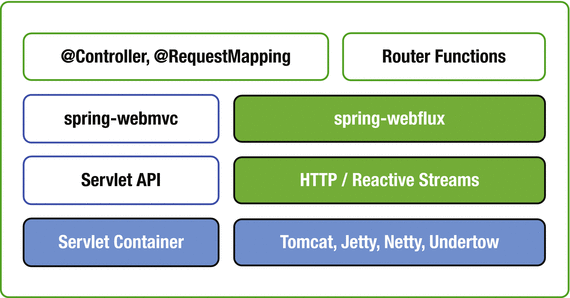
\includegraphics[width=\linewidth]{media/Spring5-runtime}
	\footref{webflux:book}    
    \label{spring5-runtime}
\end{figure}
\end{center}

WebFlux läuft grundsätzlich auf asynchronen Laufzeitumgebungen wie Tomcat, Jetty, Undertow und Netty. Es werden nur Servlet Container unterstützt, die mindestens die Servlet-Spezifikation V. 3.1 implementieren. \footref{webflux:book}

\subsection{Akka}
Akka ist ein Toolkit, daher eine Sammlung von Bibliotheken, mit dem sich Reactive Systeme realisieren lassen. Das heißt, dass Technologien die entsprechend dem  \autoref{sec:das_reaktive_manfiest} notwendig sind, bereits im Repertoire von Akka sind. Die folgende Tabelle fasst einige Akka Module zusammen.

\begin{table}[H]
\caption{Unvollständige Liste der Akka Module}
\centering
\begin{tabular}{|l|l|}
\hline
\rowcolor[HTML]{00A99D} 
{\color[HTML]{FFFFFF} Akka Modul}      & {\color[HTML]{FFFFFF} Beschreibung}                                                                                                              \\ \hline
Actors           & \begin{tabular}[c]{@{}l@{}}Implementierung des Aktorenmodells\\ zur nachrichtenbasierten Kommunikation\end{tabular}       \\ \hline
Streams          & \begin{tabular}[c]{@{}l@{}}Für nicht-blockierende und nebenläufige \\ Verarbeitung von Daten\end{tabular}                 \\ \hline
Cluster          & \begin{tabular}[c]{@{}l@{}}Ermöglich Skalierung und Widerstandsfähigkeit\\ durch Verteilung auf mehreren Knoten\end{tabular} \\ \hline
Distributed Data & \begin{tabular}[c]{@{}l@{}}Ermöglicht einen Lese- und Schreibzugriffe \\ mit geringer Latenzzeit auf Knoten.\end{tabular}    \\ \hline
\end{tabular}
\end{table}
\footnote{vgl. Akka Docs, \cite{web:akka:docs}}

Auf der Anwendungsebene nutzt Akka die Akka-Streams als Reactive Streams Implementierung. Prominente Unternehmen, die Akka aktiv in ihrem Production Code nutzen sind unter anderem Paypal, Twitter, Samsung, Intel, Verizon und LinkedIn. 

\subsection{Eclipse Vert.x}
Vert.X (ausgeprochen Vertex) ist ein Toolkit für nebenläufige und nicht-blockierende Anwendungen für die JVM. Das Toolkit basiert auf dem Netty Project und bietet eine High-Level API für das zugrunde liegende Netty Framework. Weiterhin ist Vert.X mehrsprachig, also ein Toolkit, dass mehrere Sprachen unterstützt, die auf der JVM laufen. Somit gibt es Support für Java, Scala, Kotlin, Groovy, Javascript, Ruby und Ceylon. \footnote{vgl. Ponge, Segismont \& Viet et al. , Seite 2-6, \cite{buch:a_gentle_guide:kapitel1} \label{vertx:intro}}

Konzeptuell hat Vert.X zwei Kernaspekte. Zum einen das Verticle und zum anderen den Eventbus. Ein Verticle ist eine Verarbeitungseinheit. Es beinhaltet eine Eventloop, in der Events entgegengenommen werden. Per Default werden zwei Verticle pro CPU Kern zur Verfügung gestellt. Der Eventbus ist für die asynchrone Kommunikation zwischen den Verticles zuständig. Zwischen Verticles wird über Nachrichten kommuniziert. Ähnlich zu Akka kann mit dem Vert.X Toolkit reaktive Systeme gebaut werden. \footref{vertx:intro}

Vert.X bietet zwei Arten von Reactive Streams an. Zum einen die Reactive Streams Integration für die Read/Write Streams, wobei es sich es um eine Überbrückung von Read/Write Stream zu Publisher/Subscriber handelt. \footnote{vgl. tsegismont, StackOverflow Kommentar \cite{web:site:stackoverflow:vertx:comment}} Zum Anderen die RxJava- Streams, allerdings wurde die Bibliothek entsprechend dem Toolkit angepasst. Das heißt es wurden einige Funktionen entfernt, die nicht mit den Modulen aus Vert.X arbeiten können. Umgekehrt wurde auch die Vert.X API an RxJava angepasst, der sogenannten Rxified API.

Bekannte Unternehmen wie Bosch, VmWare, Hulu, Zalando, Deutsche Börse Group, Red Hat und viele andere nutzen Vert.X in ihren Projekten. \footnote{vgl. Vert.X Homepage, \cite{web:site:vertx}}
\chapter{Einsatzszenarien von reaktiver Programmierung}
\label{chap:scenario}
\section{Netflix}
Netflix ist maßgeblich bei der Entwicklung von RxJava beteiligt. Die Gründe für die Entwicklung von RxJava sind im Entwicklerblog \footnote{vgl. Christensen et al., Reactive Programming in the Netflix API with RxJava \cite{web:site:medium:netflix:reactive_programming}} des Unternehmens zu finden. Der wesentliche Grund für die Entwicklung war, dass Netflix die eigene API für nebenläufige Verarbeitung optimieren wollte. Das Problem von klassischen Lösungen wie z. B. Futures und Callbacks ist, dass diese Techniken nur für einen bestimmten Grad an Nebenläufigkeit sinnvoll ist. Futures können zwar verknüpft werden und über Callbacks ein blockierendes Warten vermeiden, allerdings nimmt die Lesbarkeit mit zunehmender Komplexität stark ab. Dies bezeichnet man als Callback Hell. Da die Programmierung mit Futures und Callbacks keine langfristige Lösung für hochgradig antwortbereite Systeme ist, implementierte das Entwicklerteam von Netflix die ReactiveX API für Java. 

\section{PayPal}
Die Firma Lightbend (Akka) fasst in ihrer Fallstudie\footnote{vgl. lightbend case studies paypal \cite{web:site:lightbend:case-studies:paypal}} den Technologiewechsel des Unternehmens PayPal zusammen.
PayPal nutzt für die Verarbeitung der Transaktionen die eigens entwickelte Plattform Squbs. Die Plattform ist in Scala geschrieben und nutzt das Akka Toolkit. Die Vorteile, die Paypal durch die neue Plattform hat, sind Geschwindigkeit und eine effizientere Auslastung der Hardware. Durch die hohe Geschwindigkeit können pro Tag bis zu einer Milliarde Transaktionen verarbeitet werden. Dies erreichen sie durch acht virtuelle Maschinen mit je zwei CPU-Kernen.

Ein weiterer Vorteil ist, dass der Code im Vergleich zur Java Implementierung um ca. 80\% reduziert wurde da Scala durch seine ausdrucksstarke Syntax den Code kürzt.

Für PayPal sind unter anderem das Aktorenmodell und die Streams Bibliothek die Schlüsseltechnologien um die hohen Lasten zu verarbeiten.

\section{Verizon}
Lightbend hat in einer Fallstudie\footnote{vgl. lightbend case studies verizon \cite{web:site:lightbend:case-studies:verizon} \label{casestudy:verizon}} den Technologiewechsel des Telekommunikationsunternehmens Verizon zusammengefasst. 
Verizon nutzt die reaktive Plattform von Lightbend (Akka u. v. m.) für ihr Onlineangebot und hat laut Angaben die Verkäufe verdoppelt. Die Performance der Software wurde bei halber Hardwareauslastung verdoppelt. Mit 2,5 Milliarden Transaktionen pro Jahr ist Verizon die  am sechsthäufigsten besuchte Website in den USA.

Das alte System basierte ursprünglich auf der Oracle Commerce Platform. Ein Problem war, dass das System eine monolithische Architektur hatte. Das heißt, dass die Codebase sehr komplex und groß war. Builds und Updates mussten über Nacht kompiliert werden. Die Testumgebungen für neue Features beanspruchten zwischen fünf und zehn Tagen an Vorbereitung. In Notfällen betrug die Zeit zum Einspielen der Fixes 24 Stunden. Trotz der Probleme nahm die Anzahl an Transaktionen und Neukunden zu. Das Entwicklerteam benötigte im Schnitt zwei Monate um neue Features zu veröffentlichen.

Verizon engagierte ein Team aus Softwarearchitekten zur Erkundung von neuen Technologien als Alternative zur Oracle Comerce Platform. Zur Auswahl standen Spring Boot und Lightbend's reaktive Plattform (Akka, Play u. v. m.). Das Team entschied sich für Lightbend's reaktive Plattform da sie technische Vorteile in asynchroner Verarbeitung und I/O bieten.

Die folgende Abbildung zeigt die Gegenüberstellung des alten und neuen Systems: 

\begin{figure}[H]
\caption{Gegenüberstellung des alten und neuen Systems}
\centering
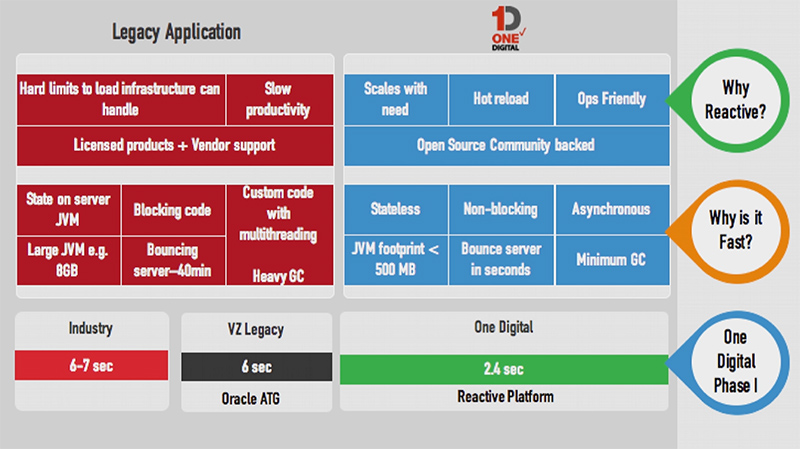
\includegraphics[scale=.5]{./media/verizon.jpg}
\footref{casestudy:verizon}
\end{figure}

Die starre Infrastruktur wurde durch eine skalierbare Infrastruktur ersetzt, die nach Bedarf Ressourcen bereitstellt. Das Entwicklungstempo wurde durch Hot Reload erhöht und ermöglicht eine insgesamt höhere Produktivität. Auf Lizenzen und Support wurde verzichtet und durch ein quelloffenes Backend ersetzt.

Die erhöhte Verarbeitungsgeschwindigkeit der Server wurde durch eine zustandlose, nicht blockierende und asynchrone Kommunikation erreicht. Der Speicherverbrauch wurde dadurch von 8 GB auf unter 500 MB gesenkt. Die Startzeit des Systems wurde von 40 Minuten auf wenige Sekunden gesenkt. Durch die Ersetzung der eigenen Multithreading Implementierung durch eine asynchrone Abstraktion wurde die Garbagecollection reduziert. 

Im direkten Performancevergleich sank die durchschnittliche Antwortzeit des neuen Systems von 6 Sekunden auf 2,4 Sekunden.

Die Verkäufe nahmen um 235\% zu und die \gls{Konversionsrate} stieg um 197\%. Aus technischer Sicht benötigt das neue System 40\% weniger Bauzeit und hat insgesamt 50\% weniger Kosten als das Vorgängersystem. 



%
% Teil 3. Konzeption und Realisierung einer Anwendung
%
\chapter{Konzeption einer reaktiven Anwendung}
\label{chap:concept}
Die Anwendung basiert auf der Idee der Kommunikation zwischen autonomen Fahrzeugen und Servern. Ein Fahrzeug misst die Signalstärke eines Signals zum nächsten Mobilfunkmast und sendet einem Server die Signalstärke sowie die aktuelle Position in Form von Koordinaten. Der Server verarbeitet die Daten und sendet dem Fahrzeug eine Antwort. Mit den gewonnenen Datan (Signalstärke und Koordinate) lassen sich nun Heatmaps erzeugen, also bspw. eine  Stadtkarte die farblich markierte Bereiche anzeigt, in denen autonome Fahrzeuge, ohne Verbindungsabbruch, fahren können. 

Die Anwendung soll die Kommunikation zwischen Server und Fahrzeug reaktiv umsetzen. Anschließend sollen ein Vergleich zu einer blockierenden Variante gezogen werden.

\section{Anforderungen}
Die prototypische Anwendung muss folgende Anforderungen erfüllen:
\begin{description}
\label{anforderungen}
\item [Client: ] Ein Auto fährt eine vordefinierte Route ab. Währenddessen misst es die Signalstärke zum nächsten Mast und sendet diese zusammen mit der Position an den Server. Zwischen jeder versendeten Messung wartet das Auto 200 ms.
\item [Server: ] Empfängt eine Positionskoordinate und die zugehörige Signalstärke, verarbeitet diese und sendet eine Antwort an das Auto zurück
\end{description}

\section{Die Wahl der Technologien}
Die Applikation wird in zwei Varianten implementiert. Zum einen eine reaktive und zum anderen eine synchrone, blockierende Variante.

Im Rahmen dieser Thesis wird TCP anstelle von HTTP als Übertragungsprotokoll verwendet. Der Grund dafür ist, dass eine triviale Datenstruktur (Positionskoordinate und Signalstärke) verwendet wird. Der Mehraufwand, der durch die Nutzung eines Http-Frameworks entsteht ist in diesem Fall nicht gerechtfertigt.

Für die reaktive Anwendung wird die Reactor Bibliothek verwendet, da sie unter den bekanntesten Bibliotheken am besten abschneidet (siehe Kapitel \ref{sec:bewertung}). Als Kommunikationstechnologie wird das RSocket\footnote{\href{www.rsocket.io}{www.rsocket.io}} Protokoll verwendet. Das RSocket Protokoll nutzt die Reactive Streams Semantik um Daten über verschiedenste Protokolle (TCP, UDP uvm.) zu übertragen. Die Schnittstellen sind mit denen von Reactor kompatibel.

Für die blockierende Variante wird die Socket API aus dem java.net Package verwendet, da die reaktive Version ebenfalls eine Socket Implementierung ist. 

\chapter{Umsetzung}
\label{chap:umsetzung}
\section{Die Umsetzung in RSocket und Reactor}
Der gesamte Quellcode zur Anwendung ist auf einem Github Repository unter
\url{https://github.com/Menkir/reactive-streams} zu finden.

Die folgende Tabelle zeigt die wichtigsten Klassen:
\begin{table}[H]
\centering
\caption{Klassen aus dem eigenen Prototype-Package}
\label{package:prototype}
\begin{tabular}{|l|l|}
\hline
\rowcolor[HTML]{00A99D} 
{\color[HTML]{FFFFFF} Klasse} & \multicolumn{1}{c|}{\cellcolor[HTML]{00A99D}{\color[HTML]{FFFFFF} Beschreibung}} \\ \hline
CarServer & \begin{tabular}[c]{@{}l@{}}Server der Car-Verbindungen akzeptiert\\ und die Messungen als Measurement Objekt\\ verarbeitet.\end{tabular} \\ \hline
Car & \begin{tabular}[c]{@{}l@{}}Client der eine Verbindung zum Server herstellt\\ und Measurements sendet und die Antworten\\ vom Server empfängt.\end{tabular} \\ \hline
CarConfiguration & \begin{tabular}[c]{@{}l@{}}Dient zu Konfiguration von der\\ Zeitverzögerung zwischen\\ zwei Measurements und der Route\end{tabular} \\ \hline
Measurement & \begin{tabular}[c]{@{}l@{}}Kapselt eine Koordinate als Tupel\\ und eine Signalstärke\\ als Integer Zahl.\\ Die Signalstärke wird zwischen 0 (kein Signal)\\ und 10 (volles Signal) definiert.\end{tabular} \\ \hline
IRoute & \begin{tabular}[c]{@{}l@{}}Modelliert eine Route (Abfolge von Koordinaten),\\ die ein Auto (Car) abfährt.\end{tabular} \\ \hline
Serializer & \begin{tabular}[c]{@{}l@{}}Transformiert Measurement in einen\\ Typ für den Transport zwischen Car und Server und umgekehrt.\end{tabular} \\ \hline
\end{tabular}
\end{table}

\textbf{Anmerkung zur Car Klasse:} Die reaktive als auch synchrone Variante enthalten einen internen Zähler: flowrate. Die Flowrate-Variable dient dazu, zu ermitteln wie viele erfolgreiche Messungen gesendet wurden. Eine Messung ist genau dann erfolgreich, wenn eine Car Instanz eine Messung zum Server sendet und eine Antwort erhält.

Die folgende Auflistung zeigt die wichtigsten Klassen der RSocket Bibliothek:
\begin{itemize}
\item RSocketFactory: Instantiiert Server oder Client
\item ServerRSocketFactory: Instantiiert einen Server RSocket
\item SocketAcceptor: Handler für ankommende Verbindungen
\item AbstractSocket: Definiert wie Daten übertragen werden: Request/Response, Request/Stream, Channel oder Fire-and-Forget.
\item ClientRSocketFactory: Instantiiert Client RSocket
\item RSocket: Der Socket der eine Verbindung zwischen Server und Client hält.
\item Payload: Ist ein Typ der beim Transport zwischen Client und Server verwendet wird.
\end{itemize}

\subsection{Der RSocket Server}
\label{subsection:server}
Die Server Klasse implementiert zwei Methoden: Zum einen die Receive-Methode und zum anderen die Close-Methode.
Die folgende zwei Listings zeigen zum einen die relevanten importierten Klassen, sowie die Implementierung des RSocket-Servers:

\lstinputlisting[language=Java, firstline=3, lastline=10, breaklines=true, captionpos=t, caption={Reactive Server:  Relevante Imports}, label={lst:reactive_server}]{./src/ReactiveServer.java}
\clearpage
\lstinputlisting[language=Java, firstline=35, lastline=49, breaklines=true, captionpos=t, caption={Reactive Server:  Receive-Methode aus [async.server.Server]}, label={lst:reactive_server}]{./src/ReactiveServer.java}

Im Konstruktor der Klasse wird Objekt der InetSocketAdress Klasse instantiiert. In dem Objekt sind Informationen bezüglich IP-Adresse und Port. 
Über die RSocketFactory Klasse wird der Socket konfiguriert. Die Methode acceptor (Zeile 3) enthält die Parameter der Accept-Methode aus der SocketAcceptor Klasse. Der Rückgabewert des Lambdaausdrucks muss ein Mono<RSocket> sein, da es der Rückgabewert der impliziten Accept-Methode aus SocketAcceptor ist. In Zeile 4 wird ein Mono zurückgeliefert. Das Mono enthält eine anonyme Klasse von AbstractSocket. Die anonyme AbstractSocket Klasse überschreibt die Requestchannel-Methode (Zeile 6) und gibt einen Flux vom Typ Payload zurück. Dieser Flux wird im Client subscribed.

Über die Methode transport (Zeile 12) wird das Protokoll für die Kommunikation konfiguriert. Für die Anwendung wird TCP verwendet. Die Methode start startet die Event-Loop von RSocket. Da die Event-Loop asynchron gestartet wird, kann Zeit vergehen bis der Server tatsächlich gestartet wurde. Aus diesem Grund wird blockierend über die Methode block auf einen erfolgreichen Start gewartet. 
\clearpage
Die überschriebene Methode channelRequest implementiert das Channel Interaktionsmodellen von RSocket. Insgesamt bietet RSocket vier Modelle an:

\begin{itemize}
\item Request und Response
\item Request und Stream
\item Fire-and-Forget
\item Channel
\end{itemize}

Das Channel Modell wurde gewählt da es einen bidirektionalen Kommunikationskanal zwischen Client und Server bildet. Somit lässt sich auch der Durchsatz für einen Client messen. Mit Modellen wie Request und Response oder Request und Stream wird stets ein Element übertragen und ein oder mehrere Elemente als Antwort gesendet. Das Fire-and-Forget Modell passt ebenfalls nicht in den Anwendungsfall da nur ein Element übertragen wird ohne, dass der Client eine Antwort erhält.

Die Requestchannel-Methode (Zeile 6) wird clientseitig aufgerufen. Aufgrund dessen, dass das Argument der Methode ein Publisher ist, muss er in einen allgemeinen Flux umgewandelt werden um die komfortable Reactor API zu nutzen. Über die Methode from (Zeile 7) wird ein Flux mit den Elementen aus dem Publisher erzeugt. Die Funktion flatMapSequential bewirkt, dass die Payload in ein Flux<Payload> umgewandelt wird. Dadurch ist es möglich dem inneren Flux eine Zeitverzögerung von 10 ms als Bearbeitungszeit zu geben. Die Bearbeitung eines Measurement ist daher nur eine Zeitverzögerung. Im Anschluss wird das Flux schließlich flach, daher von Flux<Flux<Payload>> zu Flux<Payload> und dem Aufrufer (Car), zurückgeliefert.

\subsection{Der RSocket Client}
Die Car Klasse implementiert die Connect-, Send- und Close-Methode. Die Connect-Methode stellt die Verbindung zwischen Car und Server her, wie folgendes Listing zeigt:

\lstinputlisting[language=Java, firstline=3 , lastline=9, breaklines=true, captionpos=t, caption={Reactive Car: Relevante Imports}, label={lst:reactive_client}]{./src/ReactiveClient.java}
\clearpage
\lstinputlisting[language=Java, firstline=51 , lastline=58, breaklines=true, captionpos=t, caption={Reactive Car: Connect-Methode aus [async.client.Car]}, label={lst:reactive_client}]{./src/ReactiveClient.java}

Über die Factory-Methode wird der Socket konfiguriert. Die KeepAliveAckTimeout-Methode setzt den Timout für eine offene Verbindung auf 30 Minuten um sicher zu gehen, dass die späteren Benchmarks ohne Verbindungsunterbrechung laufen. Als Transportprotokoll wird TCP verwendet und über ein Objekt der Klasse TcpClientTransport konfiguriert. Die Methode start und block stellen eine Verbindung her und warten blockierend (da nur eine Verbindung) auf eine erfolgreiche Verbindungsherstellung.

Die Send-Methode der reaktiven Klasse Car emittiert die Messungen von einem Car, wie folgendes Listing zeigt:

\lstinputlisting[language=Java, firstline=74, lastline=83, breaklines=true, captionpos=t, caption={Send Methode aus [async.client.Car]}, label=lst:raective:client:send]{./src/ReactiveClient.java}


Der Client RSocket frägt über die Methode channelRequest einen bidirektionalen Kanal an. Diese Methode muss serverseitig implementiert sein (Siehe Kapitel \ref{subsection:server}). Als Argument wird ein Publisher übergeben, der Elemente vom Typ Payload emittiert. Da Flux eine Implementierung des Publishers ist, wird eine Flux Instanz übergeben. Das Flux erzeugt aus einem Iterable ein Flux<Coordinate>. Das Iterable ist eine Liste von statisch definierten Koordinaten (List<Coordinate>). Über die Methode repeat (Zeile 4) wird eine Runde der Route 100.000 Mal wiederholt. Somit wird ein lang andauernder Flux simuliert, jedoch nicht unendlich. Im Rahmen dieser Anwendung wird eine festgelegte Größe emittiert da die äquivalente Socket Implementierung ebenfalls eine endliche Anzahl an Messungen versendet, denn endlose Emissionen über Sockets sind nicht möglich. Sockets benötigen stets ein Terminal, das signalisiert, dass keine Datenelemente mehr folgen. 

Die Methode delayElements (Zeile 5) verzögert die Emission der Messungen um eine definierte Zeit. Das heißt, dass zwischen zwei Messungen immer eine gewisse Zeit gewartet wird. Im Kapitel \ref{sec:benchmark} wird ein Vergleich zwischen verzögerten und nicht verzögerten Varianten gezogen. 

Die doOnNext Methode (Zeiel 6) setzt für jede Messung eine Signalstärke. Die Signalstärke wird durch eine Zahl zwischen 0 und 10 simuliert. In Zeile 7 wird jede Koordinate in eine Payload umgewandelt. Im Anschluss wird die share Methode aufgerufen, die das Flux von einem Cold-Stream in einen Hot-Stream umwandelt und somit n >= 1 Subscriber akzeptiert und die Payload im Multicast emittiert. Diese Eigenschaft ist genau dann notwendig, wenn andere Teile der Software die Daten empfangen möchten wie z. B. eine grafische Benutzeroberfläche. 

Die Subscribe-Methode in Zeile 9 erzeugt eine Subscription auf den Rückgabewert (Flux<Measurement>). Der Flux ist der Rückgabewert der auf dem Server definierten RequestChannel-Methode (siehe Listing \ref{lst:reactive_server} Zeile 6). 

Die Close Methode der reaktiven Klasse Client beendet die Subscription zwischen Client und Server:

\lstinputlisting[language=Java, firstline=88, lastline=90, breaklines=true, captionpos=t, caption={Close Methode aus async.client.Car}]{./src/ReactiveClient.java}

\section{Die Umsetzung in Socket}
Die folgende Tabelle zeigt die wichtigsten Klassen aus dem java.net Package:
\begin{table}[H]
\centering
\caption{Klassen aus dem java.net Package}
%\label{my-label}
\begin{tabular}{|l|l|}
\hline
\rowcolor[HTML]{00A99D} 
{\color[HTML]{FFFFFF} Klasse} & {\color[HTML]{FFFFFF} Beschreibung} \\ \hline
ServerSocket & Socket für den Host \\ \hline
Socket & Socket für den Client \\ \hline
ObjectInputStream & Eingangskanal für Objekte \\ \hline
ObjectOutputStream & Ausgangskanal für Objekte \\ \hline
\end{tabular}
\end{table}

Die Klassen des eignen prototype Package sind in Kapitel \ref{package:prototype} zu finden.

Der blockierende Server implementiert die receive und close Methode. Das folgende Listing zeigt die receive Methode: 
\clearpage
\lstinputlisting[language=Java, firstline=29, lastline=67, breaklines=true, captionpos=t, caption={Receive Methode aus sync.server.Server}]{./src/SyncServer.java}

Der Server lagert jeden Request in einem Future aus. Das heißt, dass eingehende Socket-Verbindungen über Threads asynchron verarbeitet werden. Innerhalb des Future werden über den InputStream vom Server die Messungen blockierend und synchron empfangen. Anschließend werden die Messungen unverändert an den Client über den OutputStream des Server zurückgesendet.

Die Car Klasse implementiert die connect, send und close Methode. Das folgende Listing zeigt die connect Methode:

\lstinputlisting[language=Java, firstline=50, lastline=58, breaklines=true, captionpos=t, caption={Connect Methode aus sync.client.Car}]{./src/SyncClient.java}

Zuerst wird eine Socket Instanz erzeugt und anschließend über die Methode connect mit dem Server verbunden. Der Paramter in der connect Methode enthält die Informationen zu IP und Port.

Das folgende Listing zeigt die öffentliche send und die private sendData Methode:

\lstinputlisting[language=Java, firstline=87, lastline=98, breaklines=true, captionpos=t, caption={Send Methode aus sync.client.Car}]{./src/SyncClient.java}
\clearpage
\lstinputlisting[language=Java, firstline=121, lastline=137, breaklines=true, captionpos=t, caption={SendData Methode aus sync.client.Car}, label=lst:sync:sendData]{./src/SyncClient.java}

Die send Methode emittiert hundert Millionen Koordinaten. In jedem Schleifendurchlauf wird eine Messung versendet, aktiv gewartet und anschließend die Prüfvariable inkrementiert. Innerhalb der sendData Methode wird ein OutputStream geöffnet und dem Server die Messung gesendet, anschließend wird über ein InputStream auf die Antwort des Servers blockierend gewartet und das Ergebnis gelesen. Zum Schluss wird die flowrate inkrementiert, die für den Benchmark benötigt wird.

Die close Methode schließt den Socket, der mit dem Server verbunden ist, wie folgendes Listing zeigt:

\lstinputlisting[language=Java, firstline=71, lastline=80, breaklines=true, captionpos=t, caption={Close Methode aus sync.client.Car}]{./src/SyncClient.java}

Wenn die Variable clientSocket eine gültige Instanz der Klasse Socket besitzt, dann darf der Socket auch über die Methode close geschlossen werden.

\section{Performance Benchmark}
\label{sec:benchmark}
Um einen qualitativen Vergleich zwischen den Varianten zu bewerkstelligen, wird der durchschnittliche Durchsatz pro Sekunde ermittelt. Hierbei entspricht der Durchsatz der Anzahl an erfolgreich übertragenen Requests. Ein Request ist genau dann erfolgreich, wenn auf ein Request eine Response empfangen wurde.

\subsection{Die Testumgebung}
Die Clients/ Fahrzeuge wurden auf einem Windows 10 Enterprise x64 Computer mit einem Intel I7 3,6 GHz Prozessor (acht CPU-Kerne) und 16 GB RAM simuliert. Der Server lief entfernt auf einem Macbook AIR6,2 (anfang 2014) mit Intel I5 1,4GHz Prozessor (vier CPU-Kernen) und 4 GB RAM. Das Testprogramm als auch der Server liefen unter der Oracle JDK Version 1.8\char`_162.

\subsection{Der Benchmark}
\label{chap:benchmark}
Es werden insgesamt zwei Benchmarks je Variante (synchron/ reaktiv) ausgeführt. Zum einen ein Benchmark mit einprogrammierter Zeitverzögerung und einmal ohne Zeitverzögerung. Der Grund weshalb Zeitverzögerungen verwendet werden ist, dass ein realistischer Test gemacht werden kann. Ein Fahrzeug entspricht einem Client. Wenn nun ein Client die maximal mögliche Anzahl an Koordinaten sendet, hat dies keine praktische Relevanz für eine Auswertung da sonst zu viele identische Messungen gesendet werden.

Der Benchmark ist in zwei Phasen unterteilt. Zum einen in eine Warmlauf-Phase und zum anderen in eine Test-Phase. In der Warmlauf-Phase werden Optimierungen vom Hotspot JIT-Compiler vorgenommen um den Code zu beschleunigen. Würde man in dieser Phase messen, zuerst anhand von nicht-optimierten und später mittels optimierten Methoden gemessen, was dazu führen würde, dass die Messungen verfälscht werden. 

Um zu gewährleisten, dass nur optimierte Methoden getestet werden, wird die JVM mit zwei Argumenten gestartet. Zum einen -client und zum anderen 
-XX:+PrintCompilation. Das erste Argument bewirkt, dass der Threshold\footnote{Bezeichnet die Anzahl an Aufrufen, die eine Methode braucht um vom JIT-Compiler optimiert zu werden.}, für die Methoden auf 1500 gesetzt wird. Das heißt, dass eine Methode 1500 mal aufgerufen werden muss um optimiert zu werden. Das zweite Argument gibt in Echtzeit die optimierten Methoden aus dem JIT-Compiler aus. \footnote{vgl. Oracle, Java HotSpot VM Options \cite{web:site:oracle:jvmhotspot}} Die Ausgabe des JIT-Compilers dient zur Verifizierung ob die Methode tatsächlich optimiert wurde.

Konkret müssen genau die Methoden optimiert werden, die für für Emission der Messungen zuständig sind da diese den Durchsatz generieren. Wenn bspw. 1000 Messungen emittiert werden, wird keine Optimierung vom JIT-Compiler vorgenommen. Der entstandene Durchsatz ist somit verfälscht. 

Da das Flux die Payload über die Reactive Streams Semantik emittiert, muss die onNext Methode optimiert werden. Jedoch wird die onNext Methode nicht explizit in der Car Klasse aufgerufen sondern implizit vom Publisher (Flux). Die folgende Abbildung zeigt die Print Ausgabe des JIT-Compilers innerhalb der Warmup Methode:

\begin{center}
\begin{figure}[H]
	\caption{Ausschnitt aus der JIT Ausgabe}
	\centering
  	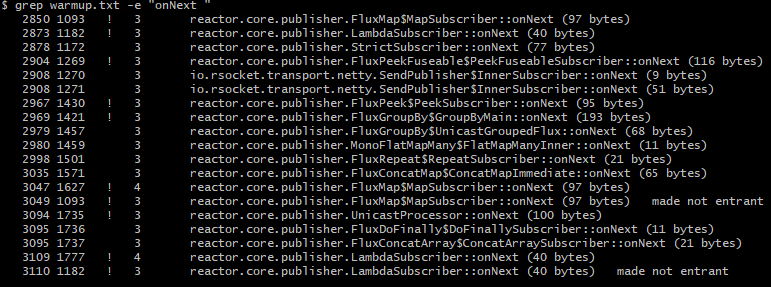
\includegraphics[width=\textwidth]{media/jit-output.png}
	\label{jit:output}
\end{figure}
\end{center}

Die erste Zeile in Abbildung \ref{jit:output} ist das FluxMap Objekt, das innerhalb der map Methode des Flux in Listing \ref{lst:raective:client:send} Zeile 7 aufgerufen wird. Da der Flux lazy evaluiert (Siehe Kapitel \ref{subsec:hotncold}) wird, beginnt der Flux erst zu senden, wenn eine Subscription erstellt wurde. Die zweite Zeile in Abbildung \ref{jit:output} ist die onNext Methode, die der Publisher beim Subscriber aufruft, wenn ein Element emittiert wird. Da der Subscriber implizit ein Lambda-Ausdruck ist, wird die onNext Methode des LambdaSubscribers aufgerufen. Hiermit wird sichergestellt, dass die Methode onNext optimiert ist. Dieses Verfahren ist analog für die synchrone Car Klasse. In der synchronen Car Klasse muss die sendData Methode geprüft werden da dort die Input- und Outputstreams aufgerufen werden, die die Messungen übertragen. (Siehe Listing \ref{lst:sync:sendData}).

\subsection{Simulation in Scala}
Die Simulationsklassen AsyncSimulation und SyncSimulation implementieren jeweils die Methoden run, warmUp und benchmark.

In der Run-Methode wird die Warmup-Methode aufgerufen, die Methoden vom JIT-Compiler optimiert. Dann werden Futures gestartet, wobei jedes Future ein Benchmark ausführt. Die Messzeit eines Benchmark steht in der durationList Liste. Anschließend wird auf das Ende aller Futures gewartet und das Resultat abgespeichert. Das folgende Listing zeigt die Implementierung der Run-Methode aus der AsyncSimulation Klasse:

\lstinputlisting[language=Scala, firstline=28, lastline=38, breaklines=true, captionpos=t, caption={Run Methode aus der AsyncSimulation Klasse}]{./src/AsyncSimulation.scala}

Die Warmup-Methode: 

\lstinputlisting[language=Scala, firstline=65, lastline=76, breaklines=true, captionpos=t, caption={Warmup Methode aus der AsyncSimulation Klasse}]{./src/AsyncSimulation.scala}

Wie in Kapitel \ref{chap:benchmark} beschrieben, werden 1500 Koordinaten als Request gesendet und empfangen um die Methoden der Bibliothek zu optimieren.
\clearpage
Die Benchmark-Methode:

\lstinputlisting[language=Scala, firstline=47, lastline=57, breaklines=true, captionpos=t, caption={Benchmark Methode aus der AsyncSimulation Klasse}]{./src/AsyncSimulation.scala}

In der Methode wird eine Client Instanz erzeugt und gestartet. In der asynchronen Variante ist die send() Methode nicht-blockierend. In Zeile 6 schläft der Thread die notwendige Measuretime-Zeit während das Car die Messungen sendet und den Durchsatz Zähler (flowcounter) inkrementiert. Anschließend die Instanz mit der Methode close beendet und die Variable flowcounter zurückgeliefert.

Die Simulation wird aus der folgenden Main Methode gestartet:

\lstinputlisting[language=Scala, firstline=80, lastline=84, breaklines=true, captionpos=t, caption={Main Methode aus der AsyncSimulation Klasse}]{./src/AsyncSimulation.scala}

Die SyncSimulation Klasse unterscheidet sich im wesentlichen nur darin, dass das Senden des Car in einem Future ausgelagert wird. Der restliche Code ist analog und im Anhang \ref{chap:programming:test:sync} zu finden.
\clearpage
\subsection{Auswertung der Testergebnisse}
\subsubsection{Messung mit Verzögerung}
Bei der ersten Messung wurde eine Sendeverzögerung im CarConfiguration Objekt von 200 ms gesetzt. Somit folgt, dass ein durchschnittlicher Durchsatz von 5 Koordinaten pro Sekunde als optimal gilt.

Die folgende Abbildung zeigt die Messung der reaktiven und synchronen Anwendung mit Sendeverzögerung.
\begin{center}
\begin{figure}[H]
	\caption{Messung mit Zeitverzögerung}
	\centering
  	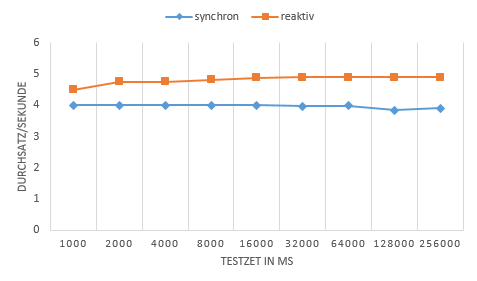
\includegraphics[width=\textwidth]{media/messung_mit_delay}
	\label{messung_mit_delay}
\end{figure}
\end{center}

Die folgende Tabelle zeigt den Durchsatz beider Varianten: 

\begin{table}[H]
\centering
\caption{Messung mit Zeitverzögerung (tabellarisch)}
\label{benchmark:withdelay}
\begin{tabular}{l|l|l|l|l|}
\cline{2-5}
 & \multicolumn{2}{l|}{\cellcolor[HTML]{00A99D}{\color[HTML]{FFFFFF} Reakitv}} & \multicolumn{2}{l|}{\cellcolor[HTML]{00A99D}{\color[HTML]{FFFFFF} Synchron}} \\ \hline
\rowcolor[HTML]{00A99D} 
\multicolumn{1}{|l|}{\cellcolor[HTML]{00A99D}{\color[HTML]{FFFFFF} Messzeit in ms}} & \multicolumn{4}{l|}{\cellcolor[HTML]{00A99D}{\color[HTML]{FFFFFF} Durchsatz / Skunde}} \\ \hline
\multicolumn{1}{|l|}{1000} & \multicolumn{2}{l|}{4} & \multicolumn{2}{l|}{0} \\ \hline
\multicolumn{1}{|l|}{2000} & \multicolumn{2}{l|}{4,5} & \multicolumn{2}{l|}{4} \\ \hline
\multicolumn{1}{|l|}{4000} & \multicolumn{2}{l|}{4,75} & \multicolumn{2}{l|}{4} \\ \hline
\multicolumn{1}{|l|}{8000} & \multicolumn{2}{l|}{4,75} & \multicolumn{2}{l|}{4} \\ \hline
\multicolumn{1}{|l|}{16000} & \multicolumn{2}{l|}{4,8125} & \multicolumn{2}{l|}{4} \\ \hline
\multicolumn{1}{|l|}{32000} & \multicolumn{2}{l|}{4,875} & \multicolumn{2}{l|}{4} \\ \hline
\multicolumn{1}{|l|}{64000} & \multicolumn{2}{l|}{4,890625} & \multicolumn{2}{l|}{3,96875} \\ \hline
\multicolumn{1}{|l|}{128000} & \multicolumn{2}{l|}{4,890625} & \multicolumn{2}{l|}{3,976563} \\ \hline
\multicolumn{1}{|l|}{256000} & \multicolumn{2}{l|}{4,890625} & \multicolumn{2}{l|}{3,835938} \\ \hline
\multicolumn{1}{|l|}{512000} & \multicolumn{2}{l|}{4,894531} & \multicolumn{2}{l|}{3,90625} \\ \hline
\end{tabular}
\end{table}

Die reaktive Variante strebt einen Wert von 5 an und ist somit näher am optimalen Durchsatz als die synchrone Variante. Der Grund weshalb die synchrone Variante einen geringeren Durchsatz hat ist, dass die zusätzlich zu der Verzögerung des Car (200 ms) noch auf die Antwort des Servers warten muss. Da der Server 10 ms braucht um eine Messung zu verarbeiten, muss ein synchrones Car mindestens 210 ms warten. Die folgende Abbildung demonstriert die Kommunikation zwischen Server und Car in der reaktiven und synchronen Variante:
\begin{center}
\begin{figure}
\caption{Reaktive Car und Server Kommunikation mit Sendeverzögerung}
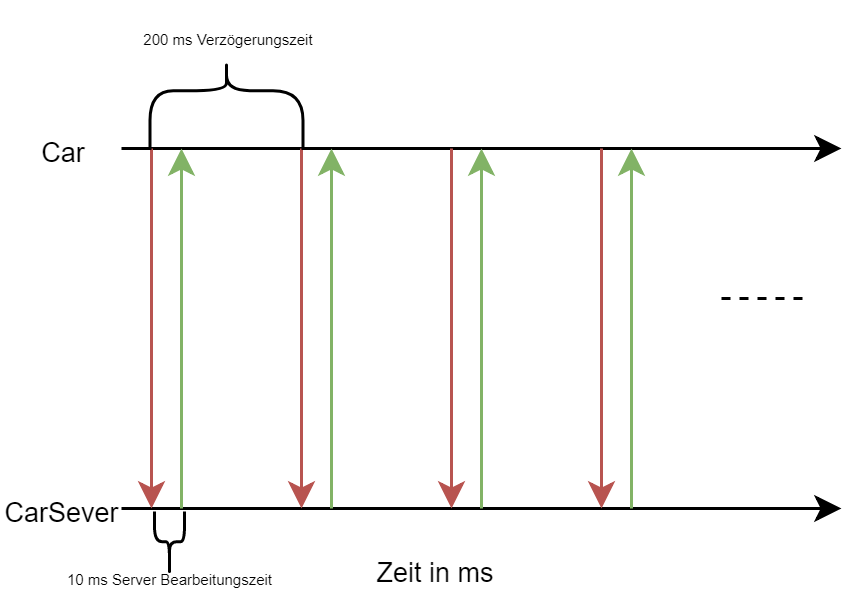
\includegraphics[scale=.5]{./media/with_delay_reactive.png}
\caption{Synchrone Car und Server Kommunikation mit Sendeverzögerung}
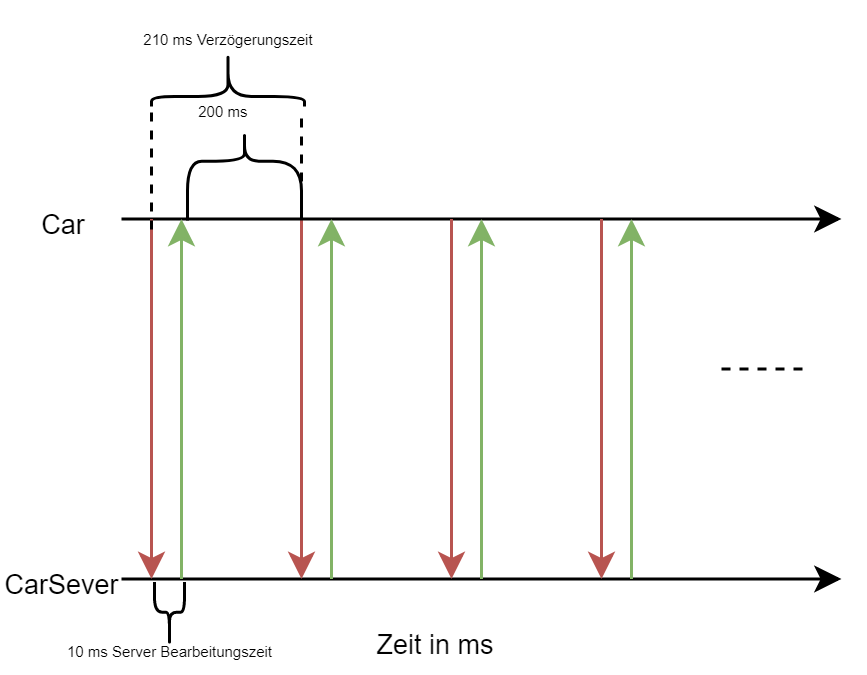
\includegraphics[scale=.5]{./media/with_delay_synchron.png}
\end{figure}
\end{center}

\clearpage
\subsubsection{Messung ohne Verzögerung}
Die Messung ohne Verzögerung soll die Bedingungen eines Servers unter Last simulieren, indem alle Clients so viele Messungen senden wie möglich. Die folgende Abbildung zeigt die Messung ohne Verzögerung, wobei der Maßstab unterschiedlich ist, da die reaktive Variante einen stark erhöhten Durchsatz hat: 

\begin{center}
\begin{figure}[H]
	\caption{Messung ohne Zeitverzögerung}
	\centering
  	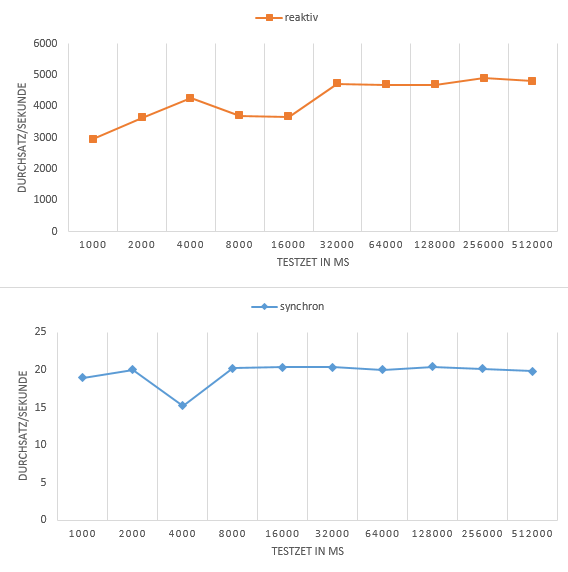
\includegraphics[width=\textwidth]{media/messung_ohne_delay}
	\label{messung_ohne_delay}
\end{figure}
\end{center}

Die reaktive Anwendung strebt einen konstanten Durchsatz von 5000 an während die synchrone Anwendung einen Durchsatz von 20 erreicht. Die folgende Tabelle zeigt den Duchsatz pro Sekunde für die synchrone und reaktive Variante:

\begin{table}[H]
\centering
\caption{Messung ohne Zeitverzögerun (tabellarisch)}
\label{benchmark:withoutdelay}
\begin{tabular}{l|l|l|}
\cline{2-3}
 & \cellcolor[HTML]{00A99D}{\color[HTML]{FFFFFF} Reaktiv} & \cellcolor[HTML]{00A99D}{\color[HTML]{FFFFFF} Synchron} \\ \hline
\rowcolor[HTML]{00A99D} 
\multicolumn{1}{|l|}{\cellcolor[HTML]{00A99D}{\color[HTML]{FFFFFF} Messzeit in ms}} & \multicolumn{2}{l|}{\cellcolor[HTML]{00A99D}{\color[HTML]{FFFFFF} Durchsatz / Sekunde}} \\ \hline
\multicolumn{1}{|l|}{1000} & 2948 & 19 \\ \hline
\multicolumn{1}{|l|}{2000} & 3636,5 & 20 \\ \hline
\multicolumn{1}{|l|}{4000} & 4262,5 & 15,25 \\ \hline
\multicolumn{1}{|l|}{8000} & 3701,75 & 20,25 \\ \hline
\multicolumn{1}{|l|}{16000} & 3675,375 & 20,375 \\ \hline
\multicolumn{1}{|l|}{32000} & 4727,15625 & 20,375 \\ \hline
\multicolumn{1}{|l|}{64000} & 4696,484375 & 20,015625 \\ \hline
\multicolumn{1}{|l|}{128000} & 4683,921875 & 20,4375 \\ \hline
\multicolumn{1}{|l|}{256000} & 4906,941406 & 20,148438 \\ \hline
\multicolumn{1}{|l|}{512000} & 4797,521484 & 19,818359 \\ \hline
\end{tabular}
\end{table}

Die hohe Differenz des Durchsatzes zwischen der reaktiven und der synchronen Variante entsteht dadurch, dass ein reaktives Car nicht-blockierend auf die Antwort des Servers wartet. Dadurch sendet das Car so viele Messungen wie möglich. Die reaktive Implementierung sendet bereits während der Bearbeitungszeit des Servers weitere Anfragen, sodass ein höherer Durchsatz möglich ist. Die folgende, Abbildung demonstriert die Kommunikation zwischen Car und Server in reaktiver als auch synchroner Variante: 

\begin{center}
\begin{figure}[H]
\caption{Reaktive Car und Server Kommunikation ohne Sendeverzögerung}
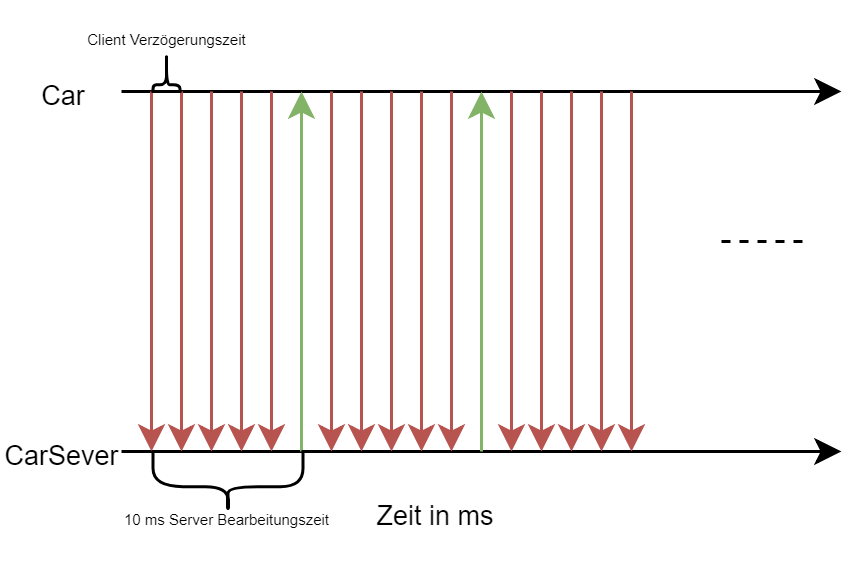
\includegraphics[scale=.5]{./media/without_delay_reactive.png}

\caption{Synchrone Car und Server Kommunikation ohne Sendeverzögerung}
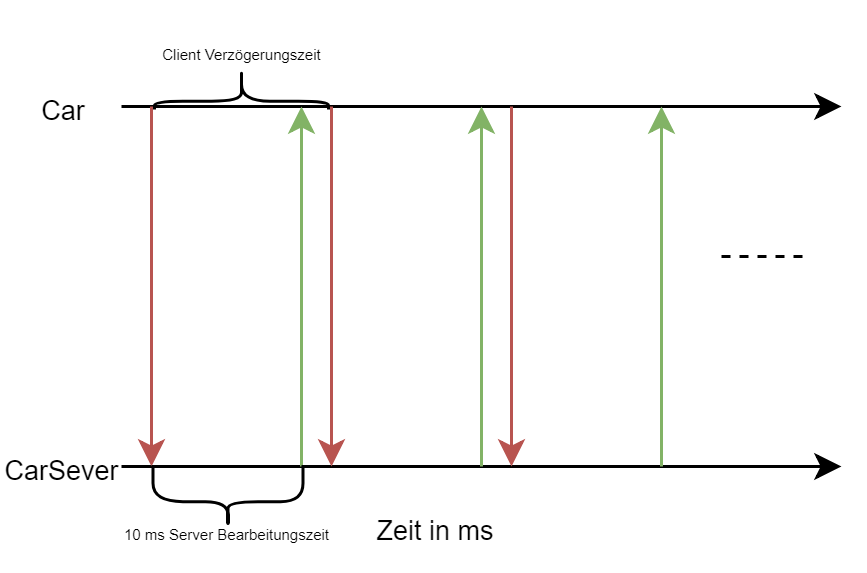
\includegraphics[scale=.5]{./media/without_delay_synchron.png}
\end{figure}
\end{center}

\subsubsection{Ergebnis}
Die reaktive Implementierung ist deutlich performanter wie die synchrone Variante. Ohne Sendeverzögerung kann ein Client mehr als 4500 Messungen mehr versenden als ein synchroner Client. Die Geschwindigkeit ergibt sich maßgeblich aus dem blockierenden Verhalten der Anwendung. Selbst unter gedrosselten Bedingungen (200 ms Sendeverzögerung) schafft der reaktive Client einen Durchsatz nahe am Optimum.
%
% CHAPTER Fazit
%
\chapter{Fazit}
\label{chap:fazit}
Reaktivität ist ein Begriff der im wesentlichen in zwei Bereichen der Softwareentwicklung stark an Popularität gewonnen hat. Zum einen in reaktiven Systemen und zum anderen in reaktiver Programmierung. Während ein reaktives System eine Architektur beschreibt, die eine hochgradig antwortbereite Systeme ermöglicht, meint die reaktive Programmierung ein Programmierparadigma, mit dem asynchrone und nicht-blockierende Anwendungen entwickelt werden können. 

Die Streams sind als de facto Standard in der reaktiven Programmierung anzusehen, denn sie haben wie das reaktive Manifest ebenfalls eine Standardisierung, die Reactive Streams Specification. Anders wie Streams aus der Collection API von Java, können reactive Streams nicht-blockierend Daten mit Back Pressure verarbeiten. Das ermöglicht eine Skalierung in vertikaler Ebene, die mit den Java Streams nicht ohne weiteres nicht möglich ist. So gibt es zwar Techniken wie Futures, die sogar Teilaspekte der Reactive Streams anbieten. Allerdings können Futures keine Sequenzen von Daten übertragen und müssen den Rückgabewert über Callback-Funktionen verarbeiten. Diese Art der Verarbeitung führt häufig zur so genannten Callback-Hell. Reactive Streams lösen diese Probleme, jedoch bietet sich deren Verwendung nicht in jedem Fall an. Sind einzelne Anfragen und blockierender Code nützlicher, sollte überlegt werden, ob sich der erhöhte Lernaufwand für den Anwendungsfall lohnt. In Anwendungen, die parallel und nicht-blockierend laufen, lassen sich mit Reactive Streams verständliche und übersichtliche Algorithmen entwickeln. \\

Vorreiter auf dem Gebiet der Reactive Streams in Java ist Netflix durch die Entwicklung der RxJava Bibliothek. Diese implementiert die Reactive Streams Specification und vereinfacht die nebenläufige Programmierung durch eine deklarative API maßgeblich. In der Android-Welt erfreut sich RxJava großer Beliebtheit und gilt dort als Standardbibliothek für reaktive Programmierung. Unternehmen wie Pivotal und Lightbend bieten mit ähnlichen Bibliotheken wie etwa Reactor3 und Akka-Streams (als Teil von Akka) Alternativen. \\

Von den drei betrachteten Bibliotheken erwies sich Reactor als einsteigerfreundlichste und am besten bedien- und benutzbare Bibliothek. Dabei zeichnet sich Reactor vor allem durch eine schlanke API und eine verständliche Dokumentation aus. Allerdings ist diese Bibliothek nicht so weit verbreitet und findet vorzugsweise in Spring-Projekten Anwendung. Zu den reaktiven Bibliotheken gibt es allerdings auch Frameworks, die mehrere Technologien in sich vereinen und es sogar ermöglichen, ganze reaktive Systeme im Sinne des reaktiven Manifests zu bauen. Das beliebteste Framework unter Entwicklern ist hierbei Spring, das im Webflux Modul die Reactor-Bibliothek nutzt und in Konkurrenz zu Akka und VertX steht. Besonders Akka hat in den letzten Jahren stark an Popularität gewonnen, da es als Toolkit eine große Auswahl an Modulen aufweist und mit Scala eine Alternative zu Java bietet. \\

Die Entwicklung des reaktiven Prototyps zeigt im Wesentlichen zwei Dinge auf: Zum einen sind reaktive Programme komfortabler zu programmieren, zum anderen sind sie performanter als blockierende Programme. \\

Zusammengefasst lässt sich sagen, dass reaktive Programmierung eine moderne und sichere Art ist, nebenläufig zu programmieren. Reaktive Bibliotheken sind bereits Teil der größten Frameworks auf dem Markt und ermöglichen es, stabile reaktive Systeme zu bauen. Es ist zu erwarten, dass der Trend zur reaktiven Programmierung weiter anhält und den Standard für nebenläufige, nicht-blockierende Anwendungen setzt. \\

 Nicht zuletzt ist auch die Tatsache, dass die Java 9 Flow-Api als fester Bestandteil in das JDK aufgenommen wurde, ein deutlicher Indikator für die momentane und künftige Bedeutung der reaktiven Programmierung. 


%% Use letters for the chapter numbers of the appendices.
\appendix
\chapter*{Anhang}
\label{chap:APPENDIX}
\addcontentsline{toc}{chapter}{Anhang}
%\setcounter{chapter}{0}
\addtocounter{chapter}{1}
\setcounter{section}{0}
\section{Quellcode}
\label{chap:APPENDIX_SOURCECODE}
\subsection{Reactive Server Implementierung}
\lstinputlisting[language=Java, breaklines=true, captionpos=t, caption={Reactve Server Implementation}, label={reactive:server:impl}]{./src/ReactiveServer.java}
\subsection{Reactive Client Implementierung}
\lstinputlisting[language=Java, breaklines=true, captionpos=t, caption={Reactive Client Implementation}, label={reactive:client:impl}]{./src/ReactiveClient.java}
\subsection{Socket Server Implementierung}
\label{chap:programming:sync:server}
\lstinputlisting[language=Java, breaklines=true, captionpos=t, caption={Socket Server Implementation}, label={blocking:server:impl}]{./src/SyncServer.java}
\subsection{Socket Client Implementierung}
\label{chap:programming:sync:client}
\lstinputlisting[language=Java, breaklines=true, captionpos=t, caption={Socket Client Implementation}, label={blocking:client:impl}]{./src/SyncClient.java}
\subsection{Test der reaktiven Variante}
\label{chap:programming:test:async}
\lstinputlisting[language=Scala, breaklines=true, captionpos=t, caption={Scalatest der reaktiven Variante}]{./src/AsyncSimulation.scala}
\subsection{Test der synchronen Variante}
\label{chap:programming:test:sync}
\lstinputlisting[language=Scala, breaklines=true, captionpos=t, caption={Scalatest der synchronen Variante}]{./src/SyncSimulation.scala}

\printbibliography[heading=bibintoc]

\end{document}
%------------------------------------
% ╔═╗╔╗╔╔╦╗  ╔╦╗╔═╗╔═╗╦ ╦╔╦╗╔═╗╔╗╔╔╦╗
% ║╣ ║║║ ║║   ║║║ ║║  ║ ║║║║║╣ ║║║ ║ 
% ╚═╝╝╚╝═╩╝  ═╩╝╚═╝╚═╝╚═╝╩ ╩╚═╝╝╚╝ ╩ 
%------------------------------------
